%  $Author: awl8049 
%  $Date: 2011/12/13 17:51:16 $
%  $Revision: 3.6 $
%
\documentclass[prodmode,acmtaco,pdftex]{acmsmall}
\usepackage[nocompress]{cite}
% Set variables used by the graphicx package (included in acmsmall)
\DeclareGraphicsExtensions{.png,.jpg}
% Packages used to produce document
\usepackage[cmex10]{amsmath}
\interdisplaylinepenalty=2500
\usepackage{array}
\usepackage{url}
\usepackage[caption=false,labelfont=sf,textfont=sf,captionskip=5pt]{subfig}
\usepackage{fixltx2e}
\newcommand{\equationname}{Eq.}
\newcommand{\equationnames}{Eqs.}
\newcommand{\figurenames}{Figs.}
\newcommand{\figurename}{Fig.}
\hyphenation{op-tical net-works semi-conductor}
\acmVolume{V}
\acmNumber{N}
\acmArticle{A}
\acmYear{2012}
\acmMonth{5}
\begin{document}
\markboth{Adam Wade Lewis, et. al}{Run-Time Energy Consumption
  Estimation for Server Workloads based on Chaotic Time-Series Approximation }
\title{Run-Time Energy Consumption
  Estimation for Server Workloads based on Chaotic Time-Series Approximation} 
\author{ADAM WADE LEWIS, NIAN-FENG TZENG, and SOUMIK GHOSH
\affil{University of Louisiana at Lafayette}}
\begin{abstract}
  This paper proposes a run-time model which relates server energy
  consumption to its overall thermal envelope, using hardware
  performance counters and experimental measurements.  While previous
  studies have attempted system-wide modeling of server power
  consumption through subsystem models, our approach is different in
  that it links system energy input to subsystem energy consumption
  based on a small set of tightly correlated parameters.  The proposed
  model takes into account processor power, bus activities, and system
  ambient temperature for real-time prediction on the power consumption
  of long running jobs.  Using the HyperTransport and QuickPath Link
  structures as case studies and through electrical measurements on
  example server subsystems, we develop a chaotic time--series
  approximation for run-time power consumption, arriving at the Chaotic
  Attractor Predictor (CAP).  With polynomial time complexity, CAP
  exhibits high prediction accuracy, having the prediction errors within
  1.6\% (or 3.3\%) for servers based on the HyperTransport bus (or the
  QuickPath Links), as verified by a set of common processor benchmarks.
  Our CAP is a superior predictive mechanism over existing linear
  auto-regressive methods, which require expensive and complex
  corrective steps to address the non-linear and chaotic aspects of the
  underlying physical system.
\end{abstract}
\category{B.8}{\textbf{Hardware}}{PERFORMANCE AND RELIABILITY}
\category{C.4}{\textbf{Computer systems Organization}}{PERFORMANCE OF
  SYSTEMS} 
\category{D.4.8}{\textbf{Operating Systems}}{Performance}
\terms{Measurement, Performance, Reliability} 
\keywords{Analysis of variance, chaotic time series, energy consumption,
  HyperTransport buses, performance counters, QuickPath links, thermal
  envelope, time series approximation} \acmformat{Lewis, A.W., Tzeng,
  N.-F., and Ghosh, S. 2012. Run-Time Energy Consumption Estimation for
  Server Workloads based on Chaotic Time-Series Approximation.}
\begin{bottomstuff}
  This journal submission is an
  extension of earlier work presented at USENIX 2010 Workshop on
  Power-Aware Systems and Computing (Hotpower'10), entitled
  "\textit{Chaotic Attractor Prediction for Server Run-Time Energy
    Consumption}" \newline%\cite{Lewis2010}. 
   \newline
  This work was supported in part by the U.S. Department of Energy (DOE)
  under Award Number DE-FG02-04ER46136 and by the Board of Regents,
  State of Louisiana, under Contract Number
  DOE-LEQSF(2004-07)-ULL. \newline
  \newline
  Authors' addresses: A.W. Lewis, Center for Advanced Computer Studies,
  University of Louisiana, Lafayette, LA 70504; e-mail:
  awlewis@cacs.louisiana.edu.  N.-F. Tzeng, Center for Advanced Computer
  Studies, University of Louisiana, Lafayette, LA 70504: e-mail:
  tzeng@cacs.ouisiana.edu.\newline
\end{bottomstuff}
\maketitle
\section{Introduction}
\label{sec:Introduction}
The upwardly spiraling operating costs of the infrastructure for
enterprise-scale computing demand efficient power management in server
environments.  It is difficult to achieve efficient power management in
data centers, as they usually over-provision their power capacity to
address the worst case scenarios. This calls for quantitatively
understanding the relationship between power consumption and thermal
envelope at the system level so as to optimize the use of deployed power
capacity in the data center.

Current AMD and Intel processors employ different techniques for
processor-level power management ~\cite{AMD2008b,Intel2009}. In general,
those techniques take advantage of the fact that reducing switching
activity within the processor lowers energy consumption, and that
application performance can be adjusted to utilize otherwise idle time
slacks on the processor for energy savings \cite{Contreras2005}.  Power
profiles of the Intel Pentium architecture have been studied for
workstations \cite{Isci2003a,Isci2003b,Isci2006} and servers
\cite{Bircher2004,Bircher2007,Lee2005}. Recent investigation into the
power profiles of servers based on the {NUMA} architecture (for example,
the AMD64 \cite{AMD2007}, the Intel Nehalem~\cite{Intel2009}, and IBM
POWER7~ processors~\cite{Ware2010,Brochard2010}) indicates that managing
server power profiles is complicated by the existence of multiple cores
per
processor~\cite{Kansal2010,Tsirogiannis2010,Lewis2010,McCullough2011}.
As a result, this paper presents an effective full-system continuous
model with system-wide prediction of energy consumption for server
blades built on multi-core processors.

Our model treats a single server blade as one closed black-box system,
relying on the fact that measured energy input into the system can be a
function of the work done by the system (in executing its computational
tasks) and of residual thermal energy given off by the system during
execution.  It utilizes the hardware performance counters (PeCs) of the
server for relating power consumption to its consequent thermal
envelope, enabling dynamical control of the thermal footprint under
given workload.  With PeCs, the computational load of a server can be
estimated using relevant PeC readings together with a set of operating
system's performance metrics. The selection of PeCs and metrics is
guided by the observation that the computational load in processors that
use a Non-Uniform Memory Access (NUMA) architecture can be estimated by
the amount of data transferred to/from memory and amongst processors
over system buses, The result is that the underlying system is a dynamic
system whose behavior can be described as a system of deterministic
differential equations whose solution can be estimated via time-series
approximation. Our energy consumption prediction treats observed
readings of available PeCs in a discrete time series and resorts to
statistical approximation to compensate for those model components that
cannot be determined exactly.

Generally, a time series model observes past outcomes of a
physical phenomenon to anticipate future values of that
phenomenon.  Many time series-based models of processor energy
consumption have been considered
\cite{Rivoire2008a,Bhattacharjee2009,Powell2009,Reich2010,Bircher2011},
with recent work extending such models into the thermal domain
\cite{Coskun2008}.  Time series are typically handled in three broad
classes of mechanisms: auto-regressive, integrated, and moving average
models \cite{Box1994}.  Each of these classes assumes a \textit{linear
relationship} between the dependent variable(s) and previous data
points. However, energy consumption, ambient temperature, processor die
temperatures, and CPU utilization in computers can be affected by more
than just past values of those measurements made in isolation from each
other~\cite{Bertran2010,McCullough2011}.  Our analysis of experimental
measurements of key processor PeC readings and performance metrics
reveals that the measured readings and metrics of a server over the time
series do not possess linearity and are \textit{chaotic in nature}.
This chaotic nature may result from the behavior of various server components,
like DC-DC switching power converters commonly used by power circuitry in modern
computers~\cite{Hamill1997,Tse2002}.
It thus leads to our development of a Chaotic Attractor Predictor (CAP)
that models the dynamics of the underlying system of differential equations.

Servers based on the HyperTransport bus \cite{HT2008} and the Intel
QuickPath Links \cite{Intel2009} are chosen as representatives to validate
our CAP for estimating run-time power consumption.  CAP takes into
account key thermal indicators (like ambient temperatures and die
temperatures) and system performance metrics (like performance counters)
for system energy consumption estimation within a given power and
thermal envelope. It captures the chaotic dynamics of a server system
without complex and time-consuming corrective steps usually required by
linear prediction to account for the effects of non-linear and chaotic
behavior in the system, exhibiting polynomial time complexity.  This
work demonstrates that appropriate provision of additional PeCs beyond
what are provided by a typical server is required to obtain more
accurate prediction of system-wide energy consumption.

\section{Prior Work}
\label{sec:priorwork}
Used to guide power management mechanisms in server systems, power
models can be classified into two broad categories: simulation-based and
analytical models. Although simulation may provide details and
breakdowns of energy consumption, it is usually done statically in an
off-line manner, is slow, and does not scale well nor apply favorably to
realistic applications and large data sets. For example, the HotSpot
thermal simulator \cite{Skadron2004} models thermal behavior (and,
indirectly, power behavior) by building a network of thermal resistances
and capacitances to account for heating and power dissipation on a
circuit.Such models must accurately reflect empirical data from the real
systems being simulated. Studies of the power characteristics of the
SPEC CPU 2000 and CPU 2006 benchmarks suites executed on the AMD Athlon
64 processor \cite{MesaMartinez2007} and thermal \cite{MesaMartinez2010}
show that simulation-based models (1) need long execution times to
accurately predict power behavior and (2) have problems dealing with key
thermal metrics.  Mercury \cite{Heath2006} attempts to address these
issues by adopting a hybrid approach with an out-of-band solver that
processes component observations collected from a monitor daemon on the
target system.  The solver in this system uses the collected information
to simulate the thermal behavior in the system.  The Mercury
infrastructure was used to construct Freon and FreonEC for thermal and
energy management of clusters. However, statistical analysis of methods
similar to those used in Freon indicate significant issues in this case
\cite{DavisRivoire2011}. Therefore, simulation-based models are
unsuitable when dynamic power and thermal optimization are
concerned~\cite{Economou2006}.
 
Analytical models, by contrast, rely on power measurements at the
constituent components of a server via sampling its hardware and
software performance metrics, i.e., processor PeCs (performance
counters) and operating system performance metrics.  PeCs are hardware
registers that can be configured to count various micro-architectural
events, such as branch mis-predictions and cache misses.  Attempts have
been made to reconcile analytic models by mapping program phases to
events \cite{Isci2006}.  Common techniques for associating PeCs and/or
performance metrics with energy consumption adopt linear regression to
map collected metrics to energy consumed during program execution
\cite{Contreras2005,Economou2006,Isci2003b}.

Models have been built for the processor, storage devices, single
systems, and groups of systems in data
centers~\cite{Kadayif2001,Isci2003b}.  For example, memory manufacturers
provide clear architectural documentation concerning the power
consumption of their products \cite{Micron2007}; this information is
regularly used as the foundation for modeling DRAM power
usage~\cite{Liu2008,Lewis2008}.  Similarly, detailed thermal and power
models of storage devices \cite{Gurumurthi2005} have been proposed.
However, those models considered only the maximum internal data rate,
thereby inadequate for our purpose of run-time measurement.  At the
processor level, Bellosa \citeyear{Bellosa2003} and Contreras \textit{et
  al.}  \citeyear{Contreras2005} created power models which linearly
correlated power consumption with PeCs.  Those models are simple and
fast with low-overhead~\cite{Bircher2007,Powell2009,Bircher2011}, but
they are sensitive to benchmarks chosen for model calibration and often
suffer from large worst-case errors, making them unsuitable for
predictive purposes~\cite{McCullough2011}.  Furthermore, they do not
consider full-system power consumption.

The black-box approach, without detailed knowledge of underlying
hardware, has been applied recently to full-system modeling
\cite{Bircher2007,Bircher2011} by using PeCs to estimate power
consumption of I/O devices, in addition to the processor.  In general,
full-system models can be created using operating system CPU
utilization~\cite{Fan2007} and similar metrics~\cite{Heath2005} in
addition to PeCs. Such
full-system models, like MANTIS~\cite{Economou2006,Rivoire2008a} and
trickle-down power modeling \cite{Bircher2011}, relate usage information
to the power of the entire system rather than of its individual
components.  Each of those models requires one or more calibration
phases to determine the contribution of each system component to overall
power consumption.  The accuracy and the portability of full system
power models were assessed earlier~\cite{Rivoire2008b}, revealing that
reasonable accuracy across machines and different workloads was
achievable by considering both PeCs (performance counters) and operating
system performance metrics, since they together may capture all
components of system dynamic power consumption.

Auto-regressive (AR) techniques have been adopted popularly to construct
power and temperature models for servers
\cite{Coskun2008,Powell2009,Bircher2011}, since they are simple and
efficient.  The linear AR models attempt to correlate PeCs to system
behavior, with an average error of five to twenty-five percent
(depending on architecture and benchmarks).  Unfortunately, their
maximum errors tend to be ill-conditioned, because of their
\textit{stationary} nature.  In a stationary process, the probability
distribution does not change with time, nor do the mean and the
variance.  Hence, AR and auto-regressive/moving average (ARMA) models
are not suited for data that exhibits sudden bursts of large amplitudes
at irregular time epochs, due to their assumptions of
normality~\cite{Tong1993}.  Given workload dynamics of a server vary in
time and its power profiles often diverge over time, effort has been
made to accommodate this diverse behavior
\cite{MesaMartinez2007,Coskun2008} so as to permit continuing use of AR
and ARMA models.  This way, however, negatively impacts the performance
advantage resulting from auto-regressive techniques, namely, their
simplicity.

Lately, the power consumption data collected during benchmark execution
have signified their increasing non-linearity over time. For example,
analysis of published results for the SPECpower\_ssj2008
benchmark~\cite{Varsampoulos2010,Hsu2011} revealed maximum errors as
large as 40\% when modeling the benchmark results using linear two-point
interpolation with the observation that the behavior of the power curves
of this benchmark was neither linear nor convex.  A variation of the
MANTIS power model \cite{Economou2006} was used to analyze the power
curves of the SPEC CPU2006, PARSEC multi-threaded benchmark
suite~\cite{Bienia2011}, and a set of synthetic system stress
benchmarks~\cite{McCullough2011}.  This work found for multi-core
processors that the mean relative error doubled as compared to when the
benchmark was restricted to executing on a single core.  Furthermore,
mean relative errors for individual subsystems such as the CPU were
significantly higher, with an average error of 10-14\% and the largest
error as much as 150\% for some workloads.

The cause of non-linear behavior in power data may be attributed to a
number of factors.  First, while the assumption of linearity depends
upon homogeneous workloads, observations of the behavior of SPEC CPU
benchmarks in both physical and virtual machine environments reveal that
distributing execution tasks across multi-core processors is rarely
uniform to have homogeneous workloads~\cite{Kansal2010}.  Second, modern
processors have no simple features which can be abstracted
easily to permit linear models (for example, effects such as cache
contention, processor performance optimizations, and hidden device
states) ~\cite{McCullough2011}.

Dealing with workload dynamics without high computational complexity
requires efficient estimation able to address inherent non-linearity in
the time series.  One approach follows local polynomial fitting via
weighted least squares regression \cite{Fan1996} or its variation
\cite{Singh2009}.  Another approach is to utilize a moving average
technique for smoothing the data by computing an average of the a subset
of data from the time series observations.  For example, an
exponentially-weighted moving average will weight the members of the
subset in geometrically decreasing order so as give less weight to
samples as they are further removed in time \cite{NIST2010}. A third
approach to fitting non-linear curves with varying degrees of smoothness
in different locations makes use of the derivatives of an approximating
function with discontinuities.  This can be accomplished by employing
splines with discontinuities existing at points identified as knots.  An
example of this approach is Multivariate Adaptive Regression Splines
(MARS) \cite{Friedman1991}, which models the time series as a weighted
sum of basis functions $B_{i}(x)$ and constant coefficients $c_{i}$:
\begin{equation}
  \label{eq:mars}
  f(x)= \displaystyle\sum_{i=1}^{k}c_{i}B_{i}(x),
\end{equation}
where each of the basis functions can take the form of (1) a constant 1,
with only one such term present, the intercept, (2) a hinge function in
the form of $max(0,x - c)$ or $max(0, c - x)$, or (3) a product of two or
more hinge functions.   MARS is suitable for modeling power
behavior because of their good balance between bias and variance.
A model with low bias signifies that it is flexible enough to address
non-linearity while sufficiently constrained to maintain low variance.
More details about MARS can be found in Appendix.

Chaotic systems are ubiquitous in nature, found in many different
physical domains.  One key feature of such a
dynamic system is its sensitivity to initial conditions, whose small
difference $\delta{x}$ can result in the marked difference of
$\delta{x}e^{\lambda t}$ after time $t$, for a certain $\lambda > 0$.
This exponential separation signifies that even a small difference or
error may lead to large divergence in the near future.

From a mathematical standpoint, chaos can be produced by both continuous
and discrete systems.  A continuous system expressed by a differential
equation
\begin{equation}
  \label{eq:chaoscontinuous}
  \dfrac{dx(t)}{dt} = F(x(t)),
\end{equation}
with at least three degrees of freedom
$x(t)=[x_{1}(t),x_{2}(t),x_{3}(t),\ldots, x_{m}(t)]$,
can be related to a companion discrete system of
\begin{equation}
  \label{eq:chaosdiscrete}
  x_{n+1}=f(x_{n}),
\end{equation}
by considering \equationname~(\ref{eq:chaosdiscrete}) as a projection of
the flow for \equationname~(\ref{eq:chaoscontinuous}) on a surface.
Three conditions are necessary for such a system to show chaos: (1) the
differential equation and companion discrete system are
deterministic, (2) the functions of $f$ and $F$ must be nonlinear, and (3) the
discrete system must have a positive Lyapunov exponent~\cite{Liu2010}.

\begin{figure*}[tp]
  \begin{minipage}{0.5\linewidth}
  \centering
     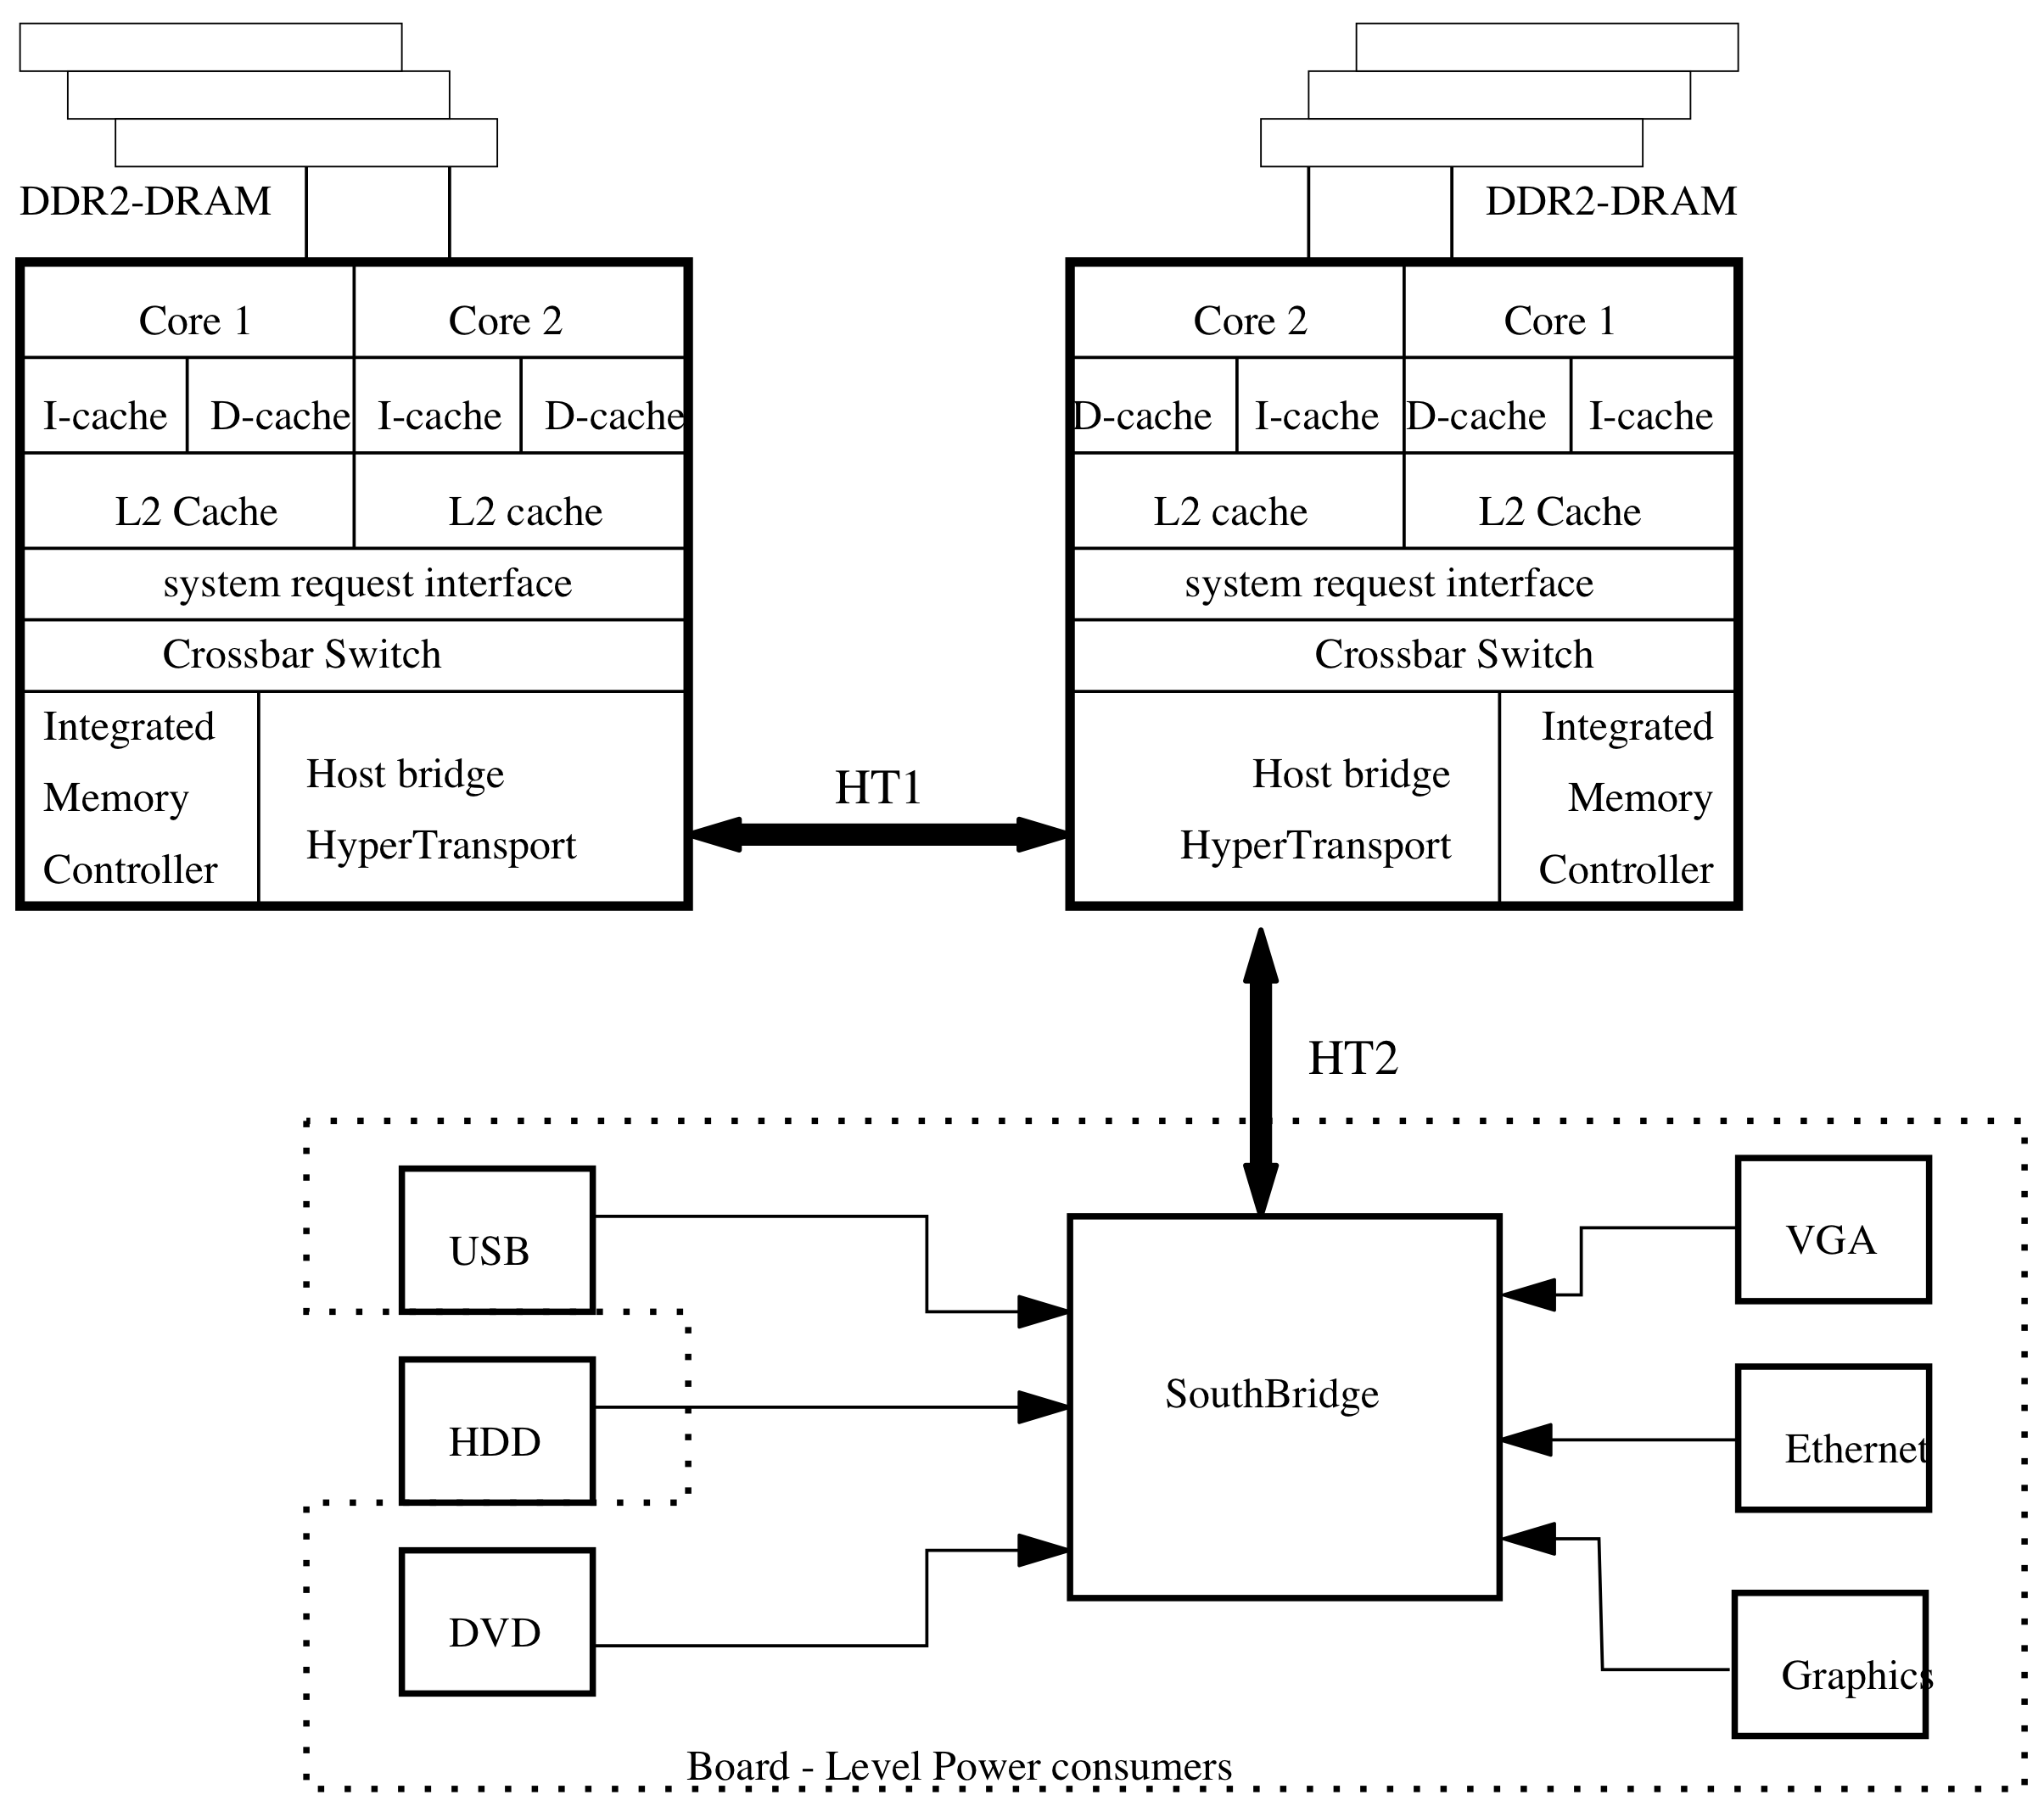
\includegraphics[scale=0.3]{x2200sys}
     \caption{AMD Opteron architecture.}
     \label{fig:amdarch}
  \end{minipage}\hspace{0.1cm}
  \begin{minipage}{0.5\linewidth}
  \centering
     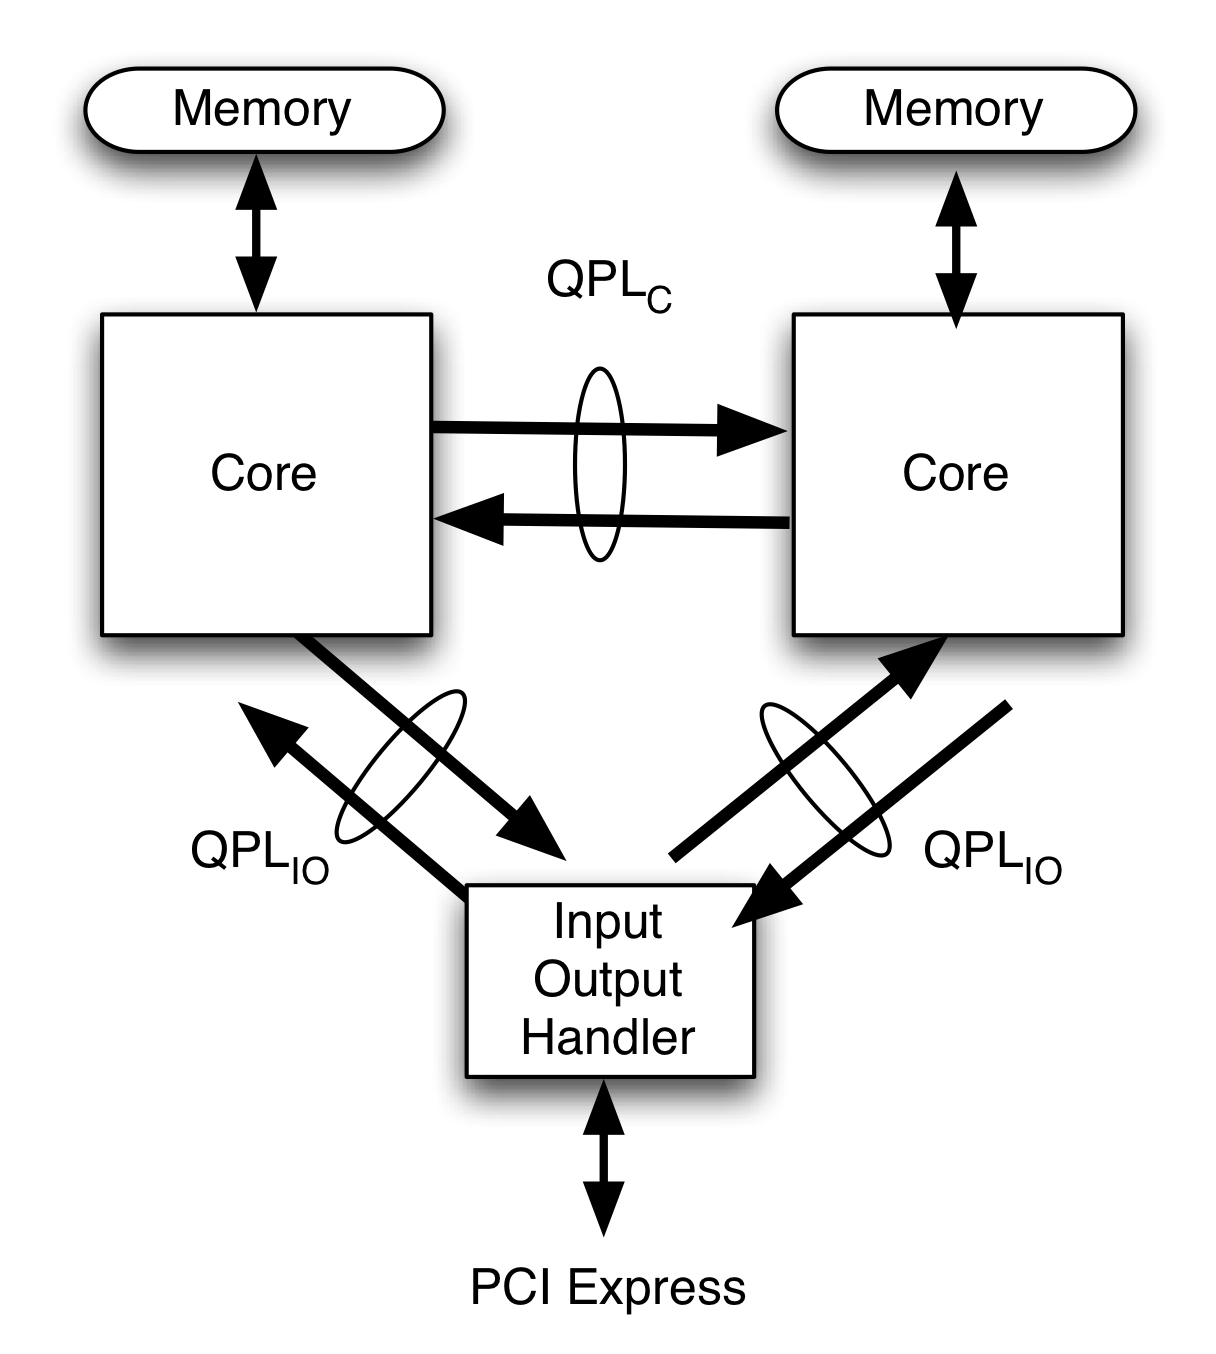
\includegraphics[scale=0.5]{intelnehalem}
     \caption{Intel Xeon (Nehalem) architecture.}
     \label{fig:intarch}
  \end{minipage}
\end{figure*}
\section{System Modeling}
\label{sec:modelstruct}
In order to develop a deterministic continuous energy consumption model
based on computational load of the system, we consider $E_{dc}$, the
total DC power input to the system, at the output of the power supply.
Most servers operate on the AC input, with efficiency of power
conversion from AC to DC equal to 72 - 80 \% (depending on the system
load~\cite{ton2008}) and with the DC output delivered in the domains of
+/-12V, +/-5V, and +/-3.3V \cite{SSI2004}.  Typically, two 12 Vdc lines
supply power to the processor's hard drive(s) and cooling fans in the
system.  The 5 Vdc and 3.3 Vdc lines are dedicated to supplying power to
the support chips and peripherals on the board.

Energy delivered to a server system, $E_{dc} = E_{system}$, can be
expressed as a sum of energy consumed by constituent sub-systems in the
server.  Generally, there are five sources of energy consumption in a
server system:
\begin{describe}{{\em $E_{board}$\/}:}
\item{$E_{proc}$:} Energy consumed in the processor due to computation,
\item{$E_{mem}$:} Energy consumed by DRAM chips,
\item{$E_{hdd}$:} Energy consumed by the hard disk drive(s),
\item{$E_{board}$:} Energy consumed by peripherals in support of board the
  operations, including all devices in multiple voltage domains across the board
  (like chip-set chips, voltage regulators, bus control chips, connectors, interface devices, etc.),
\item{$E_{em}$:} Energy consumed by all electrical and electromechanical
  components in the server, including fans and other support components.
\end{describe}

Total energy consumed by the system with a given computational workload
can be expressed as:
\begin{equation}
\label{eq:linmodel}
E_{system}= E_{proc} + E_{mem} + E_{hdd}+ E_{board} +  E_{em}.
\end{equation}
Each of the above terms is explored in turn by following an energy
conservation principle.  In order to get a true measure of the
computational load on the system, our approach snoops on bus
transactions per unit time (indicated by PeC readings), measures the
temperature changes (in die and ambient sensor readings), and records
the speeds of cooling fans, in the course of job execution.  The use of
those PeCs and metric readings fits well to NUMA-based multi-core
processors. 
\subsection{Processor energy consumption}
\label{sec:procmodel}
Consider the AMD Operton architecture and the Intel Nehalem
architecture, as depicted in \figurenames~\ref{fig:amdarch} and
\ref{fig:intarch}.  The former is a NUMA-based processor
(\figurename~\ref{fig:amdarch}), with Northbridge functionality
incorporated in the processor core and each core responsible for local
access to the memory connected to that Northbridge logic (shown in
\figurename~\ref{fig:amdarch} as ``Integrated Memory Controller'').
Processor cores on a single die are connected via a crossbar to the
HyperTransport bus (i.e., HT1) between processors.  A coherent bus
protocol is used to ensure memory consistency between processor cores on
each die.  In addition, the master processor in the system is connected
via a second HyperTransport bus (i.e., HT2) to the Southbridge device
that manages connections to the outside world.  A similar structure
exists in the Intel Xeon Nehalem architecture.  Unlike the AMD Operton,
each Nehalem processor is connected to an Input-Output handler, which
provides the Southbridge with connecting functions for off-chip resources.

It is observed that work done by any of the processors, as the heart of
energy consumption in a server system, can be quantified in terms of bus
transactions in and out of the processors.  Traffic on the external
buses provides a measure of how much data is processed by the processor.
In the case of the NUMA architecture, this quantity can be measured by
determining the amount of data transmitted over interconnect between
processor cores (HyperTransport for AMD processors, QPI links for recent
Intel processors). Our energy consumption model aims to treat each
processor as a black box, whose energy consumption is a function of its
work load (as manifested by core die temperatures measured at the system
level by \texttt{ipmitool} through sensors on the path of the outgoing
airflow from the processor).  In practice, when estimating processor
power consumption based on PeCs (performance counters), there are only a
limited number of PeCs for tools, like \texttt{cpustat}, to track
simultaneously.

For the AMD dual-core Operton architecture (shown in
\figurename~\ref{fig:amdarch}), traffic on the HT buses is viewed as a
representative of the processor workload, reflecting the amount of data
being processed by a processor (i.e., its involved cores).  The HT2 bus
is non-coherent and connects one of the two processors to the
Southbridge (whereas the Northbridge is included on the Opteron
processor die).  Thus, traffic on the HT2 bus reveals hard-disk and
network transactions.  This model scales by considering the effect of
network traffic and disk I/O transactions.  HT1 is a coherent bus
between the two SMP processors and, as such, PeCs on HT1 provide
accurate estimation on the processing load of cores executing jobs.
Per-core die temperature readings are directly affected by the number of
transactions over the HT1 bus.  A similar observation holds for the QPL
links present in the Intel Nehalem architecture, with traffic between
its two cores reflected by transactions on QuickPath Links between the
cores, denoted by $QPL_C$ (see \figurename~\ref{fig:intarch}).

Therefore, total processor power consumption at time $t$, $P_{proc}(t)$,
is related to processor temperature readings and the estimated amount of
data being processed at the time, and it can be expressed as a function
of three metrics: die temperature readings for processors 0 and 1, and
the number of bus transactions (i.e., traffic over HT1 for the AMD
server and over $QPL_C$ for the Intel server).  We have processor energy
consumption between times $t_{1}$ and $t_{2}$ as follows:
\begin{equation}
  \label{eq:procpwr2}
  E_{proc}=\displaystyle\int_{t_{1}}^{t_{2}}\left( {P_{proc}(t)} \right)dt.
\end{equation}
\subsection{DRAM energy consumption}
\label{sec:dram}
Energy consumed by the DRAM banks is directly related to the number of
DRAM read/write operations involved during the time interval of
interest, and the number is reflected by (1) the last-level cache misses
for all $N$ constituent cores ($CM_{i}(t)$, $i$ = 1, 2, ..., $N$) in
the server when executing jobs and (2) the data amount due to disk
accesses for OS support (like page tables, checkpoints, virtual
environments) and due to performance improvement for peripheral devices
(like buffered data for disks and optical devices, spooled printer
pages).  The data amount in (2) above, named $DB(t)$, is reflected by
traffic over $HT_{2}$ (or QuickPath links between the two cores and the
Input/Output handler, denoted by $QPL_{IO}$) for the AMD Opteron server
(or the Intel Xeon server), as demonstrated in
\figurename~\ref{fig:amdarch} (or \figurename~\ref{fig:intarch}).
This is because network traffic does not exist in either testing server,
which comprises only a single chip.  Additional energy contributors
include activation power and DRAM background power (due to leaking
currents), represented by $P_{ab}$.  As stated earlier
\cite{Micron2007}, DRAM activation power and background power can be
obtained from the DRAM documentation, and they together amount to 493 mW
for one DRAM module in our AMD Opteron server.  Consumed energy over the
time interval between $t_{1}$ and $t_{2}$ can be expressed by
\begin{equation*}
  \label{eq:dram}
  E_{mem}=\displaystyle\int_{t_{1}}^{t_{2}}\left( (\sum_{i=1}^{N}CM_{i}(t)+DB(t))\times
    P_{DR}+P_{ab}\right)dt,
\end{equation*} 
where $P_{DR}$ refers to DRAM read/write power per unit data.
\begin{table}%[tp]
\tbl{Hitachi HDT725025VLA360 disk power parameters\label{tab:hddparam}}{%
\begin{tabular}{ l l }
\hline
\textbf{Parameter} & \textbf{Value} \\
\hline
  Interface & Serial ATA\\
  Capacity & 250 GB\\
  Rotational speed & 7200 rpm  \\
  Power & \\
  ~~Spin up& 5.25 W (max)\\
  ~~Random read, write & 9.4 W (typical)\\
  ~~Silent read, write & 7 W (typical)\\
  ~~Idle & 5 W (typical)  \\
  ~~Low RPM idle & 2.3 W (typical for 4500 RPM)\\
  ~~Standby & 0.8 W (typical)\\
  ~~Sleep & 0.6 W (typical)\\
\hline
\end{tabular}}
\end{table}
\subsection{Hard disk energy consumption}
\label{sec:networkengery}
Energy consumed by the hard disk(s) is approximated by using a
combination of relevant PeCs and drive ratings. Building a full-system
model of disk drive energy consumption is complicated by the distance
(from the processor) and the high latency of the disk drive.  Two
earlier modeling approaches exist, with one analyzing drive performance
and capacity based on the physical characteristics of the
drive~\cite{Gurumurthi2005} and the other utilizing PeCs (which measure
DMA accesses on the memory bus, uncacheable accesses, and interrupts) to
estimate the value of $E_{hdd}$~\cite{Bircher2011}.

By contrast, our disk model is interested in the amount of information
being transferred back and forth to the device.  So, it is possible to
calculate this value using information collected by the operating system
and physical characteristics of the disk drive. Both our test servers
use the Hitachi's SATA hard disk (whose specification and relevant power
consumption figures are listed in Table ~\ref{tab:hddparam}).  Based on
the physical, electrical, and electromechanical parameters of a hard
disk, one can construct its detailed power consumption model.  However,
a cruder but simpler model can be obtained from the typical power
consumption data of hard disks and pertinent PeCs, including (1) the
number of reads and writes per second to the disk and (2) the amount of
data (in kilobytes) read from and written to the disk.  Those PeCs can
be measured by the tool of \texttt{iostat}, arriving at approximate disk
power consumption, $E_{hdd}$, as:
\begin{align*}
\label{eq:hddpwr1}
E_{hdd} = &P_{spin-up}\times T_{su}+  P_{read}\sum N_r\times T_r \nonumber\\
        &+ P_{write}\sum N_w\times T_w+ \sum P_{idle}\times T_{id}
\end{align*}
where $P_{spin-up}$ is the power required to spin-up the disk from 0 to
full rotation, and $T_{su}$ is the time required to achieve spin up,
typically about 10 sec.  $P_{read}$ (or $P_{write}$) is the power
consumed per kilobyte of data read from (or written to) the disk,
whereas $N_r$ (or $N_w$) is the number of kilobytes of data reads (or
data writes) in time-slice $T_r$ from (or to) the disk.  The Hitachi
disk achieves read operations at 1.5 Gbits/s, when consuming 530 mA
current at +5V, thereby exhibiting approximately $13.3 \mu W$/Kbyte.
Similarly, it is found to consume $6.67 \mu W$/Kbyte for write
operations.  The numbers of $N_r$ and $N_w$ can be obtained using
\texttt{iostat} according to the chosen time slice.

There are two idle states for the disk: idle and unloaded idle (when
disk read/write heads are unloaded).  The time to go from the unloaded
idle state to the idle state is usually less than 1 second (smaller than
the resolution of \texttt{iostat}).  Thus, a history match count in the
\texttt{iostat} statistics with zero reads and writes signifies the
periods in which the disk is idle, permitting us to compute idle energy
consumption accordingly.  \texttt{iostat} readings for the durations of
switching to different disk power states may be obtained with a more
in-depth analysis, which is not consider in this work.
\subsection{Board energy consumption}
\label{sec:board}
The quantity of $E_{board}$ represents energy consumption caused by the
support chipsets, control logic, buses, signal links, etc., and it
usually falls into the 3.3V and 5V power domains.  Exhibiting little
variation, $E_{board}$ can be difficult to measure, as chipset power is
drawn from multiple domains.  Hence, earlier
models~\cite{Kansal2010,Bircher2011} treated $E_{board}$ as a
constant. In our case, however, this value is obtained using current
probe-based measurements.  The results are measured over an interval of
interest, $t_{interval}$ and exclude the effects of processor, disks,
fans, and optical devices.  Note that introducing the current sensors
(possibly taking up to 28 for a server ~\cite{SSI2004}) to the power
lines on the board will provide instantaneous current readings for use
in $E_{board}$.

Aggregated power consumption effects on the board may be captured using
ambient temperature readings on the board.  Such readings can be
obtained using system management tools commonly found in server
environments (such as IPMI), and they are included in the set of our PeCs
for energy consumption estimation.
\subsection{Electromechanical energy consumption}
\label{sec:electrical}
A server always involves electromechanical energy consumption, $E_{em}$,
which is mainly due to the electromechanical functions related to system
cooling.  Multiple fans often exist in a server for cooling.  Power
drawn by the $i^{th}$ fan at time $t$ can be given by the following
equation:
\begin{equation}
\label{eq:fanp}
P_{fan}^{i}(t) = P_{base} \times \left(\frac{RPM_{fan}^{i}(t)}{RPM_{base}}\right)^3
\end{equation} 
where $P_{base}$ defines the base power consumption of the unloaded system
when running only the base operating system and no application workload.
The $P_{base}$ value is obtained experimentally by measuring the current drawn
on the +12V and +5V lines, using a current probe and an oscilloscope.
There is a current surge at system start, which is neglected.
Under nominal conditions, the +12V line draws approximately 2.2A
to power both blower fans in the AMD testing server. Total electromechanical energy consumption over a given task execution
period of $T_{p}$ equals:
\begin{equation*}
\label{eq:elect}
E_{em} =  \int^{T_{p}}_0 \left(\sum_{i=1}^NP_{fan}^{i}(t)\right)dt.
\end{equation*} 
\section{Effective Prediction}
\label{sec:application}
The current generation of server systems lacks (1)~the complete set of
measurement and monitoring capabilities and (2)~data flow state capture
mechanisms required in order to formulate the parameters of an exact
analytical model.  For example, the system board DC and AC power
consumption cannot be easily split in measurements or analyses, due to
the presence of large numbers of voltage/current domains, each with
multiple components.  Therefore, effective prediction on future power
consumption based on past power consumption readings/measurements
(obtained from PeCs and performance metrics) is critical.

In \equationname~(\ref{eq:linmodel}), $E_{system }$ signifies total
energy consumed by the system for a given computational workload, equal
to the sum of five terms: $E_{proc}$, $E_{mem}$, $E_{hdd}$, $E_{board}$,
and $E_{em}$.  Adopting \equationname~(\ref{eq:linmodel}) for server
energy consumption estimation, one needs to predict change in
$E_{system}$ over the time interval of $(t, t+\Delta t)$.  Such
prediction, following a time series to make observations of the server
system, based on PeCs and performance metrics, can be approximated by
\begin{equation}
\label{eq:tseries}
E_{system} = \hat{f}(E_{proc}, E_{mem}, E_{hdd}, E_{board}, E_{em}),
\end{equation}
where the involved parameters correspond to the five server energy
contributors modeled in Sections~\ref{sec:procmodel} to \ref{sec:electrical}.
\subsection{Performance counters and metrics}
\label{sec:variables}
In our prediction approach, fourteen (14) observable PeCs and accessible
performance metrics (referred to as "measures" collectively for simplicity)
are involved in the AMD server, as listed in Table~\ref{tab:model}.
They are grouped into five clusters, depending on their relevance to the
server energy contributors.  More specifically, the top three measures
are related to $E_{proc}$, named $MP_{proc}^{AMD} = \left[T_{C_{0}},
  T_{C_{1}}, HT_{1}\right]$.  The next five measures dictate $E_{mem}$,
denoted by $MP_{mem}^{AMD} = \left[HT_{2}, CM_{0}, CM_{1}, CM_{2},
  CM_{3}\right]$.  Those $CM_i$ measures, capturing the total L2 cache
miss counts due to Core $i$, are registered at \texttt{PAPI\_L2\_TCM} (being
OpenSolaris generic events equivalent to the matching event in the Linux
PAPI performance counter library \cite{London2001}) and mapped to the
AMD performance counters at 0x7E (as defined in \cite{AMD2008}).  The
following two measures are pertinent to $E_{hdd}$, represented by
$MP_{hdd}^{AMD} = \left[D_{r}, D_{w}\right]$, which refer to the total
numbers of bytes in disk reads and disk writes, respectively, during a
period of 5 seconds (in our experiments) for all I/O devices (which are
limited to the disk only, since no network traffic nor optical disks
exist in the two testing servers), as recorded by the system activity
monitor.  The next two measures are related to $E_{board}$, indicated by
$MP_{board}^{AMD} = \left[T_{A_0}, T_{A_1}\right]$, which register the
temperature readings of two board locations where temperature sensors
are placed.  Finally, the last two measures determine $E_{em}$, shown by
$MP_{em}^{AMD} = \left[F_C, F_M\right]$, which provide speed information
of the CPU cooling fan and the memory cooling fan.  Collectively, each
observation at time $t$ includes the 14 measures of $MP^{AMD}(t) =
\left[MP_{proc}^{AMD}, MP_{mem}^{AMD}, MP_{hdd}^{AMD},
  MP_{board}^{AMD},MP_{em}^{AMD}\right]^{T}$.
\begin{table}%[t!]
  \tbl{PeCs and performance metrics for AMD Opteron server \label{tab:model}}{%
  \begin{tabular}{r l}
\hline
\textbf{Variable}&\textbf{Measurement}\\
\hline
$T_{C_{0}}$&CPU0 Die Temp\\
$T_{C_{1}}$&CPU1 Die Temp\\
$HT_{1}$&HT1 Bus X-Actions\\
$HT_{2}$&HT2 Bus X-Actions\\
$CM_{0}$&Last-level Cache Misses due to Core0\\
$CM_{1}$&Last-level Cache Misses due to Core1\\
$CM_{2}$&Last-level Cache Misses due to Core2\\
$CM_{3}$&Last-level Cache Misses due to Core3\\
$D_{r}$&Disk bytes read\\
$D_{w}$&Disk bytes written\\
$T_{A_{0}}$&Ambient Temp0\\
$T_{A_{1}}$&Ambient Temp1\\
$F_{C}$&CPU Cooling Fan Speed\\
$F_{M}$&Memory Cooling Fan Speed\\
\hline
  \end{tabular}}
\end{table}
\begin{table}%[t!]
  \tbl{PeCs and performance metrics for Intel Nehalem server\label{tab:intelmodel}}{%
  \begin{tabular}{r l}
\hline
\textbf{Variable}&\textbf{Measurement}\\
\hline
$T_{C_{0}}$&CPU0 Die Temp\\
$T_{C_{1}}$&CPU1 Die Temp\\
$QPL_{C}$&Transactions on QPL between Cores\\
$QPL_{IO}$&Transactions on QPLs for IO Handler\\
$CM_{0}$&Last-level Cache Misses due to Core0\\
$CM_{1}$&Last-level Cache Misses due to Core1\\
$D_{r}$&Disk bytes read\\
$D_{w}$&Disk bytes written\\
$T_{A_{0}}$&Ambient Temp0\\
$T_{A_{1}}$&Ambient Temp1\\
$T_{A_{2}}$&Ambient Temp2\\
$F_{C}$&Memory Cooling Fan Speed\\
$F_{M2a}$&Memory Cooling Fan Speed 2a\\
$F_{M2b}$&Memory Cooling Fan Speed 2a\\
$F_{M3a}$&Memory Cooling Fan Speed 3a\\
$F_{M3b}$&Memory Cooling Fan Speed 3b\\
$F_{M4a}$&Memory Cooling Fan Speed 4a\\
$F_{M4b}$&Memory Cooling Fan Speed 4b\\
$F_{M5a}$&Memory Cooling Fan Speed 5a\\
$F_{M5b}$&Memory Cooling Fan Speed 5b\\
\hline
  \end{tabular}}
\end{table}

On the other hand, the Intel Nehalem server involves nineteen (19)
measures, as listed in Table~\ref{tab:intelmodel}.  Again, they are
classified into five groups, each associated with one server energy
contributor.  Notice that $QPL_{C}$ and $QPL_{IO}$ are relevant to
QuickPath Links (depicted in \figurename~\ref{fig:intarch}), and they
are associated with $E_{proc}$ and $E_{mem}$, respectively.  In
practice, however, there is just one single PeC for holding aggregated
$QPL_{C}$ and $QPL_{IO}$ together.  Among those measures listed in
Table~\ref{tab:intelmodel}, the top three are pertinent to $E_{proc}$,
comprising $MP_{proc}^{Intel}$.  The next three measures determine
$E_{mem}$, forming $MP_{mem}^{Intel}$.  Those two $CM_{i}$ measures
indicate the total L3 cache miss counts due to Core \textit{i}, $i$ = 0
or 1.  The cache miss counts record the last-level cache (i.e., L3)
misses for the Intel Xeon processor on which our testing Intel server is
built.  They are reflected by the OpenSolaris generic event,
\texttt{PAPI\_L3\_TCM} (as detailed in \cite{Sun2008b} and
\cite{Intel2009}).  The next two measures are related to $E_{hdd}$ (and
constitute $MP_{hdd}^{Intel}$), signifying the total numbers of bytes in
disk reads and disk writes, respectively, during a period of 5 seconds.
The subsequent three measures dictate $E_{board}$, obtained from 3
temperature sensors placed on the board for ambient temperature
readings; they form $MP_{board}^{Intel}$.  Finally, the last nine
measures determine $E_{em}$, offering speed information of those nine
memory cooling fans, to constitute $MP_{em}^{Intel}$.  As a result, each
observation for the Intel server at time $t$ comprises the 19 measures
of $MP^{Intel}(t) =\left[MP_{proc}^{Intel}, MP_{mem}^{Intel},
  MP_{hdd}^{Intel}, MP_{board}^{Intel}, MP_{em}^{Intel}\right]^{T}$.

A common prediction approach follows the linear auto-regressive (AR)
combination of observation measures to predict the quantities in
\equationname~(\ref{eq:tseries})  \cite{Lewis2008}.
It yields $E_{system}$ by adding up $f_{co}(MP_{co})$ for all server energy
contributors, with each $f_{co}$ (due to Contributor $co$) being a
linear summation of its constituent measures, as detailed in Appendix.
Such a linear AR approach has characteristics that make it unsuitable
for modeling server systems.  Consider the traces of actual power shown
in \figurenames~\ref{fig:compareamd} and \ref{fig:compareintel} for the
SPEC CPU2006 zeusmp benchmark as executed on an AMD Opteron or Intel
Nehalem server.  We saw indications of (1) periodic behavior and (2)
large swings in the power draw throughout the course of the benchmark run.
Similar scenarios were observed for other benchmarks on 
the AMD Opteron server and the Intel Nehalem server under this work.
Linear regression-based prediction for power draw can
mis-predict substantially (up to 44\%, as indicated in
Table~\ref{tab:modelerroroptIntel}).  Thus, it is reasonably conjectured
that \textit{non-linear dynamics} do exist in server systems.  Given
large swings in power draw usually occur to a typical server and cannot
be completely attributed to noise, more accurate prediction than linear
auto-regression and MARS \cite{Friedman1991} is indispensable.
\subsection{Chaotic prediction}
\label{sec:chaospredict}
The continuous system expressed in \equationname~(\ref{eq:linmodel}) can
be viewed as a multi-variate differential equation in the time domain
(energy being power used in a time period).  The time series
approximation of a system solution can be viewed as a projection of
the flow of \equationname~(\ref{eq:linmodel}) onto a surface~\cite{Liu2010}.
The projection is defined in a way that the behavior (i.e., energy consumption)
of the dynamic system is reflected in our discrete approximation
(i.e., our time series measures).

We performed an analysis on the data collected from our test systems to
determine if the behavior of our time series can be attributed to some
form of chaotic behavior.  A chaotic process is one which is highly
sensitive to a set of initial conditions.  Small differences in those
initial conditions yield widely diverging outcomes in such chaotic
systems.  In order to determine whether a process is chaotic, we must be
able to show that (1) it demonstrates high sensitivity to initial
conditions and topological mixing, and (2) its periodic orbits are dense
\cite{Sprott2003}.  After analyzing our experimental data, we believe
that the power consumption of a server demonstrates \textit{chaotic behavior}.

In order to evaluate a server's sensitivity to initial conditions, we
consider the Lyapunov exponents of the time series data observed while
running those benchmarks described in the previous section.  The
Lyapunov exponent quantifies the sensitivity of a system such that a
positive Lyapunov exponent indicates that the system is chaotic
\cite{Sprott2003}.  The average Lyapunov exponent can be calculated using
$\lambda = \lim_{N\to\infty}\frac{1}{N}\sum_{n=0}^{N-1}ln|f'(X_n)|$.

We found a positive Lyapunov exponent when performing this calculation
on our data set, ranging from 0.01 to 0.28 (or 0.03 to 0.35) on the AMD
(or Intel) test server, as listed in Table~\ref{tab:chaotic}, where
each pair indicates the parameter value of the AMD server followed by
that of the Intel server.  Therefore, our data has met the first and
the most significant criterion to qualify as a chaotic process.

The second indication of the chaotic behavior of the time series in
\equationname~(\ref{eq:tseries}) is an estimate of the Hurst parameter
$H$ for the data sets collected in each benchmark.  A real number in the
range of $(0, 1)$, the Hurst parameter is in the exponents of the
covariance equation for Fractional Brown motion (fBm) \cite{Sprott2003}.
If the value of the Hurst parameter is greater than $0.5$, an increment
in the random process is positively correlated and long range dependence
exists in the case of time series.  In a chaotic system, a value of $H$
approaching 1.0 indicates the presence of self-similarity in the system.
As demonstrated in Table~~\ref{tab:chaotic}, the time series data
collected in our experiments all have values of $H$ close to 1.0,
ranging from 0.93 to 0.98 (or 0.93 to 0.97) on the AMD (or Intel) test
server.
  \begin{table}%[t!]
    \tbl{Indications of chaotic behavior in power time series (AMD, Intel) \label{tab:chaotic}}{%
    \begin{tabular}{c  r r r }
      \hline
      \multicolumn{1}{c }{\textbf{Benchmark}}&\multicolumn{1}{c}{\textbf{Hurst}}&&\multicolumn{1}{c}{\textbf{Average}}\\
      \multicolumn{1}{c }{~}&\multicolumn{1}{c}{\textbf{Parameter}}&&\multicolumn{1}{c}{\textbf{Lyapunov}}\\
      \multicolumn{1}{c }{~}&\multicolumn{1}{c}{($H$)}&&\multicolumn{1}{c}{\textbf{Exponent}}\\
      \hline
      bzip2    &(0.96, 0.93)&&(0.28, 0.35)\\
      cactusADM&(0.95, 0.97)&&(0.01, 0.04)\\
      gromacs   &(0.94, 0.95)&&(0.02, 0.03)\\
      leslie3d &(0.93, 0.94)&&(0.05, 0.11)\\
      omnetpp  &(0.96, 0.97)&&(0.05, 0.06)\\
      perlbench&(0.98, 0.95)&&(0.06, 0.04)\\
      \hline
    \end{tabular}}
\end{table}

From a predictive standpoint, the unpredictable deterministic behavior
of chaotic time series means that it is difficult to build a predictor
that takes a global parametric view of the data in the series.  However,
it is possible to generate a highly accurate short-term prediction by
reconstructing the attractor in the phase space of the time series and
applying a form of least square prediction to the resulting vector space
\cite{Itoh1995,Su2010}.
\subsubsection{Chaotic Attractor Predictors}
\label{sec:capps}
With the time series introduced in \equationname~(\ref{eq:tseries}), let
$y_{t}$ be the value of $E_{system}$ at time $t$, $r$ be the total
number of PeCs and performance measures to provide metric readings, and
$X_{t}$ be the vector of those $r$ metric readings at time $t$.
According to Taken's Delay Embedding Theorem \cite{Sprott2003}, there
exists a function $\hat{f}(X_{t})$ whose behavior in the phase space
reflects the behavior of the attractors in the original time series
values $y_{t}$.  Consequently, for given $\hat{f}$, a known $X_{t}$
reveals system energy consumption at time $t$, namely, $y_{t}$.  If
$X_{t}$ can be predicted accurately for future time $t$ (likely based on
past metric readings), system energy consumption at future $t$ can be
estimated properly.  To this end, it is necessary to find a means for
approximating $\hat{f}$.

We introduce the concept of Chaotic Attractor Prediction (CAP) that
defines $\hat{f}$ in terms of least squares regression of a
multivariate local polynomial of degree $r$.  Multivariate local 
regression is a common non-parametric technique for time series
approximations.  With CAP, we extend this concept to predict the
behavior of a chaotic time series by following the approximation method
to take advantage of its polynomial time complexity while capturing the behavior
dynamics of testing systems.

Let $X$ be an observation (involving $r$ measures of 
\begin{equation*}
MP(t+\Delta t) =[MP_{proc},MP_{mem}, MP_{hdd}, MP_{board}, MP_{em}]^{T}
\end{equation*}
for a given server, as described earlier) at some future time $t+\Delta
t$ and $X_{u}$ be a prior observation (involving $r$ metric readings of
$MP(u)$) at time $u$ for $u=t-1, t-2, \dots, t-p$.  CAP localizes and
addresses the possibility of noise in our observations through
\textit{kernel weighting}.  This process starts with the standard
multivariate normal density function of $K(x)$ =
$(2\pi)^{-\frac{m}{2}}exp(-\|X\|^{2}/2)$ (where $\|X\|$ is the norm of
vector $X$) for smoothing out values of a local neighborhood, over which
our CAP is defined.  Let the bandwidth of $\beta$ be a non-negative
number and $K_{\beta}(X)$ equal $K(X/\beta)/\beta$~\cite{Fan1996}.  The
function of $K_{\beta}$ serves as a \textit{kernel} to smooth out noise
in our original observations in a non-parametric manner.  It has been
shown that $\beta$ determines the degree of smoothing produced by the
kernel~\cite{Fan2005}.  Selection of a small $\beta$ value does not
adequately address issues of noise, while a too large $\beta$ value
results in excessive bias in the results and may hide important dynamics
of the underlying function $\hat{f}$~\cite{Turlach1993}.  A preferred
choice for $\beta$ can be computed by: $\beta =
\left(\frac{4}{3p}\right)^{\frac{1}{5}}\sigma$, where $\sigma$ is the
standard deviation of observed values, estimated via the formula of
$\bar{\sigma}$ = $median(|x_{i}-\bar{\mu}|)/0.6745$, with $\bar{\mu}$
being the median of observed values ~\cite{Bowman1997}.
 
An approximation for $\hat{f}$ is defined subsequently in terms of
a locally weighted average \cite{Box1994,Fan1996} over the next
$n$ observations, based on the prior $p$ observations of $X_{t-1},
\ldots, X_{u}, \ldots, X_{t-p}$ (each with $r$ measures, namely,
$MP(u) = \left[MP_{proc}, MP_{mem}, MP_{hdd}, MP_{board}, MP_{em}\right]^{T}$,
as described earlier):
  \begin{equation}
    \label{eq:localconst}
    \hat{f}(X)=\dfrac{\displaystyle\sum_{d=t}^{t+n-1}O_{p}*K_{\beta}(X_{d}-X)}{\displaystyle\sum_{d=t}^{t+n-1}K_{\beta}(X_{d}-X)}\nonumber
  \end{equation}
with $O_{p}=(X_{t-1}, X_{t-2}, \ldots, X_{t-p})$.
 
The process can be improved by defining a local approximation
via applying a truncated Taylor series expansion of $\hat{f}(X)$ for $X$ at nearby $x$:

  \begin{equation}
    \label{eq:localtaylor}
    \hat{f}(X)=\hat{f}(x)+\hat{f}^{'}(x)^{T}(X-x).\nonumber
  \end{equation}

The coefficients of the polynomial $\hat{f}$ are then determined by minimizing
  \begin{equation}
    \label{eq:lsq}
    \displaystyle\sum_{d=t}^{t+n-1}\left(X_{d}-a-b^{T}(X_{d}-x)\right)^{2}*K_{\beta}(X_{d}-x).
  \end{equation}
 with respect to $a$ and $b$, which are estimators to
$\hat{f}(x)$ and $\hat{f}'(x)$, respectively.  The predictor generated
by solving \equationname~(\ref{eq:lsq}) can be explicitly written, according to
\cite{Box1994}, as
  \begin{equation}
    \label{eq:locallin}
    \hat{f}(x)=\frac{1}{n}\displaystyle\sum_{d=t}^{t+n-1}(s_{2}-s_{1}*(x-X_{d}))^{2}* K_{\beta}((x-X_{d})/\beta)
  \end{equation}
with $s_{i}=\frac{1}{n}\displaystyle\sum_{d=t}^{t+n-1}(x-X_{d})^{i}*K_{\beta}((x-X_{d})/\beta)$, for $i$ = 1 or 2.
\subsubsection{CAP Creation}
\label{sec:cappcreate}
There are three steps involved in the process of creating a CAP predictor:
(1) creating a training set for the process, (2) using the
observations from the training set to find the appropriate delay
embedding using Takens Theorem and then apply the nearest neighbors
algorithm in the embedded set to identify the attractors, and (3)
solving the resulting linear least squares problem that arises from
applying \equationname~(\ref{eq:lsq}) to the attractors using the
function expressed by \equationname~(\ref{eq:locallin}).

\begin{table}%[t!]
  \tbl{SPEC CPU2006 benchmarks used for model calibration\label{tab:specbenchs}}{%
  \begin{tabular}{c c p{5cm}}
    \hline
    \multicolumn{3}{l}{\textbf{Integer Benchmarks}} \\
    \hline
    bzip2&C&Compression\\
    mcf&C&Combinatorial Optimization\\
    omnetpp&C++&Discrete Event Simulation\\
    \multicolumn{3}{l}{\textbf{FP Benchmarks}} \\
    \hline
    gromacs&C/F90&Biochemistry/Molecular Dynamics\\
    cactusADM&C/F90&Physics/General Relativity\\
    leslie3d&F90&Fluid Dynamics\\
    lbm&C&Fluid Dynamics\\
    \hline
  \end{tabular}}
\end{table}
The training set for the predictor is constructed from a consolidated
time series created by executing the SPEC CPU2006~\cite{spec2006}
benchmarks listed in Table~\ref{tab:specbenchs} on target systems.  The
benchmarks were selected using two criteria: sufficient coverage of the
functional units in the processor and reasonable applicability to the
problem space.  Components of the processor affect the thermal envelope
in different ways~\cite{Kumar2008}.  This issue is addressed by
balancing the benchmark selection between integer and floating point
benchmarks in the SPEC CPU2006 benchmark suite.  Second, the benchmarks
were selected from the suite based upon fit into the problem space.
Each benchmark represents an application typical of the problems solved
on high-performance application servers.  

Each benchmark in the calibration set was executed with a sampling
interval of $t=5$ seconds.  The observations from each time interval
were consolidated on this time interval using two methods: arithmetic
mean (average) and geometric mean.  Trial models were constructed using
each method and a statistical analysis of variance indicated that time
series generated from the geometric mean
produced the best fit to the collected data.
   
\subsubsection{Time Complexity}  
The time complexity of creating a predictor is governed by the third
step in the process.  The task of reconstructing the state space by
delay embedding is linear in time as one must make up to $d$ passes
through the observations, under the embedding dimension of $d$.
Thus, the time required is $O(dn)$, where $n$ is the number of future
observations.  Then, it becomes a matter of applying a naive form of
$k^{th}$ nearest neighbors algorithm to identify the points in the
attractors.  This step involves finding the squared distance of all the
points in the nearest analogs in the Takens set and then sorting the
result to determine the $d$-nearest neighbors.  This step takes
$O(n\log{n}+n)$.  The high cost of computing the linear least squares
solution in the third step is avoided by using the explicit expression
given in \equationname~(\ref{eq:locallin}).  The time complexity of computing this
expression can be shown to be $O(n*n)$, with $O(n)$ due to computing
$s_{i}$, for $i$ = 1 or 2.  As a result, the time complexity for
establishing a CAP predictor equals $O(n^{2})$.  It should be noted that
the construction of a CAP predictor is done only once for a given
server, irrespective of applications executed on the server.  Such
construction is based on past PeC observations (totally, $p$ of them)
to predict the future PeC readings.  As $p$ grows (with more past PeC
observations involved), the time complexity of CAP increases linearly,
as can be obtained in \equationname~(\ref{eq:lsq}).  The actual computation time
results under different $n$ and $p$ values for our CAP code implemented
using MATLAB are provided in the next section.
\begin{figure}[tp]
    \centering
    %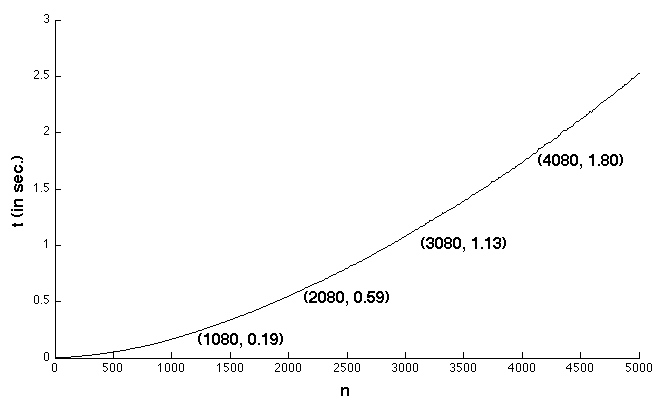
\includegraphics[scale=0.6]{complexity}
    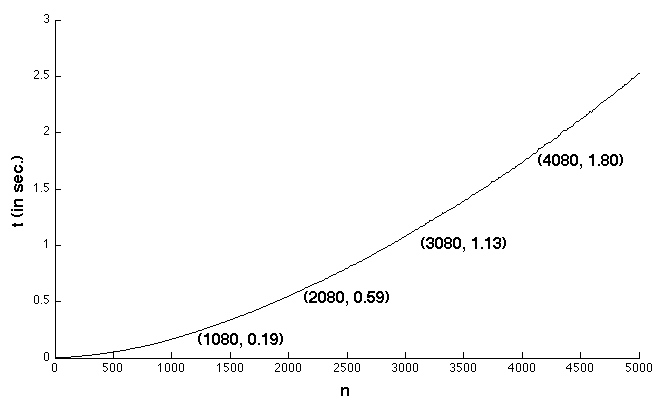
\includegraphics[width=0.9\linewidth,height=2.5in]{complexity}
    \caption{CAP time complexity versus no. of future observations.}
    \label{fig:complexity}
\end{figure}
\hspace{0.3cm}
\begin{figure}
    \centering
%    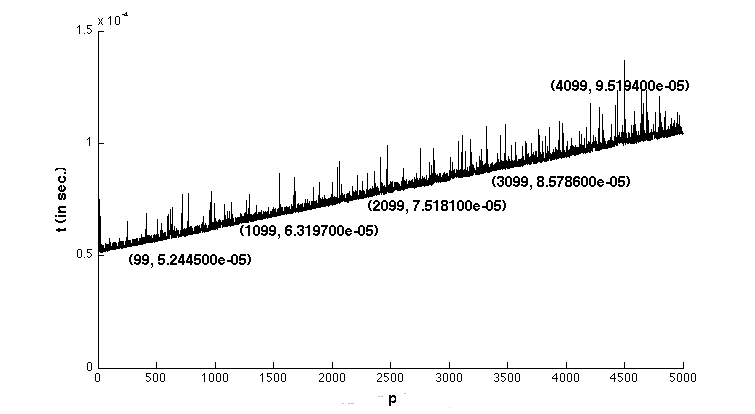
\includegraphics[scale=0.6]{complexity_p}
    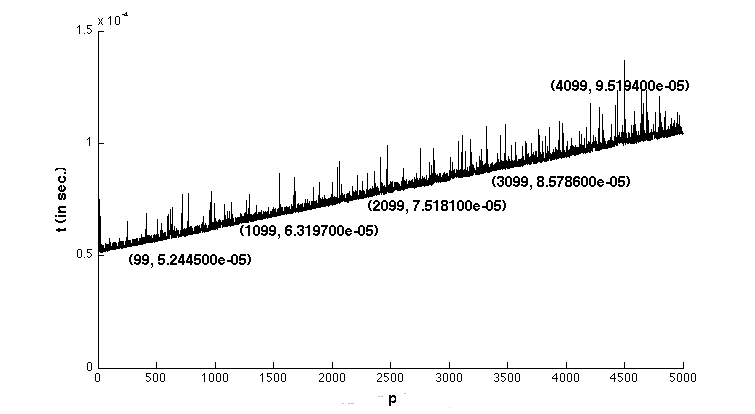
\includegraphics[width=1.0\linewidth,height=2.5in]{complexity_p}
    \caption{CAP time complexity versus no. of past observations.}
    \label{fig:complexityp}
\end{figure}
\section{Evaluation and Results}
\label{sec:evaluation}
Experiments were carried out to evaluate the performance of the CAP
power models built for approximating dynamic system solutions.  The
first experiment aimed to confirm the time complexity of CAP.  Making
use of MATLAB, our CAP code was executed on the two servers specified in
Table~\ref{tab:hardware}.  As the execution times on both servers
provide the same trend, only those collected from the SUN Fire 2200
server (AMD Opteron) are demonstrated here.  The code execution time
results versus $n$ (the number of future observations) is illustrated in
\figurename~\ref{fig:complexity}, where the result curve confirms CAP
time complexity in $O(n^{2})$.  Separately, the CAP execution time as a
function of $p$ (the number of past observations) on the SUN Fire server
is shown in \figurename~\ref{fig:complexityp}, where the time indeed is
linear with respect to $p$, as claimed earlier in our time complexity
subsection.  In practice, a moderate $p$ (of, say, 100) and a small $n$
(of, say, 5) may be chosen under CAP for high accuracy and very low time
complexity in real-time applications.  The results of distant future
(corresponding to a larger $n$) can be predicted by a step-wise process,
with each step predicting the near future outcomes (using $n$ = 5).
\begin{figure*}[tp]
  \centering
  \includegraphics[scale=0.15]{hwtestsetup2}
  \caption{Hardware test setup.}
  \label{fig:hardware}
\end{figure*}
\begin{table}%[tbhp]
  \tbl{Server configurations for evaluation\label{tab:hardware}}{%
  \begin{tabular}{l l l}
   \hline
    &\textbf{Sun Fire 2200}&\textbf{Dell PowerEdge R610}\\  
    \hline
    CPU&2 AMD Opteron&2 Intel Xeon (Nehalem) 5500\\
    CPU L2 cache&2x2MB&4MB\\
    Memory&8GB&9GB\\
    Internal disk&2060GB&500GB\\
    Network&2x1000Mbps&1x1000Mbps\\
    Video&On-board&NVIDA Quadro FX4600\\
    Height&1 rack unit&1 rack unit\\
    \hline
  \end{tabular}}
\end{table}
\subsection{Evaluation environment}
\label{sec:measurementtools}
The operating system used in our test servers is OpenSolaris (namely,
Solaris 11).  Evaluation results are collected from the system baseboard
controller using the IPMI interface via the OpenSolaris
\texttt{ipmitool} utility.  Processor performance counters are collected
on a system-wide basis by means of \texttt{cpustat}, \texttt{iostat},
and \texttt{ipmitool} utilities in OpenSolaris.  Of these,
\texttt{iostat} and \texttt{ipmitool} are available across all
UNIX-based operating systems commonly employed by data centers, while
\texttt{cpustat} is an OpenSolaris-specific utility (which is being
ported to Linux).
\begin{table}%[tbp]
  \tbl{SPEC CPU2006 benchmarks used for evaluation\label{tab:addspec}}{%
  \begin{tabular}{c c p{5cm}}
    \hline
    \multicolumn{3}{l}{\textbf{Integer Benchmark}} \\
    \hline
    Astar&C++&Path Finding\\
    Gobmk&C~~&Artificial Intelligence: Go\\
    \multicolumn{3}{l}{\textbf{FP Benchmarks}} \\
    \hline
    Gamess&F90&Quantum chemical computations\\
    Zeusmp&F90&Computational Fluid Dynamics\\
    \hline
  \end{tabular}}
\end{table}

Four benchmarks from the SPEC CPU2006 benchmark suite were used for the
evaluation purpose, as listed in Table~\ref{tab:addspec}), and they are
different from those employed earlier for CAP creation (as listed in
Table V). It is noted that selection of benchmarks for both calibration
and evaluation were selected to sufficiently exercise processor, cache,
and memory again per the decision criteria in \cite{Phansalkar2007},
with the additional criterion of selecting workloads more common to
server environments. As illustrated in Table~\ref{tab:benchstats}
(per results from \cite{Phansalkar2007}), the mix of instructions
exercises the key components of processor, memory, and cache in the
dynamic system which we model with CAP. In addition, the four
benchmarks used in our evaluation represent the type of high-utilization
workloads in server environments per typical industry use of the SPEC
CPU2006 benchmark suite \cite{Cisco2010}.
\begin{table}%[tbph]
  \tbl{Branch and Memory Access Patters of Evaluation Benchmarks\label{tab:benchstats}}{%
\begin{tabular}{lllllrrr}
\hline
% BEGIN RECEIVE ORGTBL perfmetrics
Benchmark & Inst Count & Branches & Loads & Stores \\
 & (Billions) &  &  &  \\
\hline
astar & 1,200 & 15.57\% & 40.34\% & 13.75\% \\
gamess & 5,189 & 7.45\% & 45.87\% & 12.98\% \\
gobmk & 1,603 & 19.51\% & 29.72\% & 15.25\% \\
zeusmp & 1,566 & 4.05\% & 36.22\% & 11.98\% \\
\hline
% END RECEIVE ORGTBL perfmetrics
\end{tabular}}
\end{table}

The benchmarks were executed on the two servers specified in
Table~\ref{tab:hardware}, with performance metrics gathered during the
course of execution.  Power consumed is measured by a WattsUP power meter
\cite{WattsUp2006a}, connected between the AC Main and the server under
test (SUT).  The power meter measures the total and average wattage,
voltage, and amperage over the run of a workload.  The internal memory
of the power meter is cleared at the start of each run and the measures
collected during the runs are downloaded (after execution completion)
from meter's internal memory into a spreadsheet.  Current flow on
different voltage domains in the server is measured using an Agilent
MSO6014A oscilloscope, with one Agilent 1146A current probe per server
power domain (12v, 5v, and 3.3v).  This data was collected from the
oscilloscope at the end of each benchmark execution on a server and then
stored in a spreadsheet on the test host.
{\addtolength{\tabcolsep}{-3pt}
\begin{table}%[thbp]
  \tbl{Model errors for CAP (under $n=5$, $p=100$, $r=14$), AR(1),
    MARS, and EWMA on AMD Opteron server\label{tab:modelerroropt}}}&\multicolumn{1}{c}{\textbf{Err \%}}&\multicolumn{1}{c|}{}&\multicolumn{1}{c}{\textbf{Err \%}}&\multicolumn{1}{c}{\textbf{Err \%}}&\multicolumn{1}{c }{\textbf{}}\\
        \hline
      Astar &0.9\%&5.5\%&0.72&3.1\%&8.9\%&2.26\\
      Gamess&1.0\%&6.8\%&2.06&2.2\%&9.3\%&2.06\\
      Gobmk &1.6\%&5.9\%&2.30&1.7\%&9.0\%&2.30\\
      Zeusmp&1.0\%&5.6\%&2.14&2.8\%&8.1\%&2.14\\
      \hline
      \multicolumn{1}{c|}{}&\multicolumn{3}{c|}{\textbf{MARS}}&\multicolumn{3}{c}{\textbf{EWMA}}\\
      \hline
  &\multicolumn{1}{c}{\textbf{Avg}}&\multicolumn{1}{c}{\textbf{Max}}&\multicolumn{1}{c|}{\textbf{RMSE}}&\multicolumn{1}{c}{\textbf{Avg}}&\multicolumn{1}{c}{\textbf{Max}}&\multicolumn{1}{c}{\textbf{RMSE}}\\
\multicolumn{1}{c|}{\textbf{Benchmark}}&\multicolumn{1}{c}{\textbf{Err \%}}&\multicolumn{1}{c}{\textbf{Err \%}}&\multicolumn{1}{c|}{}&\multicolumn{1}{c}{\textbf{Err \%}}&\multicolumn{1}{c}{\textbf{Err \%}}&\multicolumn{1}{c }{\textbf{}}\\
      \hline
      Astar &2.5\%&9.3\%&2.12&1.2\%&7.9\%&2.40\\
      Gamess &3.0\%&9.7\%&2.44&1.1\%&7.8\%&1.42\\
      Gobmk &3.0\%&9.1\%&2.36&1.0\%&6.9\%&2.30\\
      Zeusmp&2.8\%&7.9\%&2.34&1.8\%&9.2\%&2.01\\
      \hline
    \end{tabular}}
  \end{table}
}
\subsection{Results}
\label{sec:htcase}
\begin{figure}[tp]
  \centering
  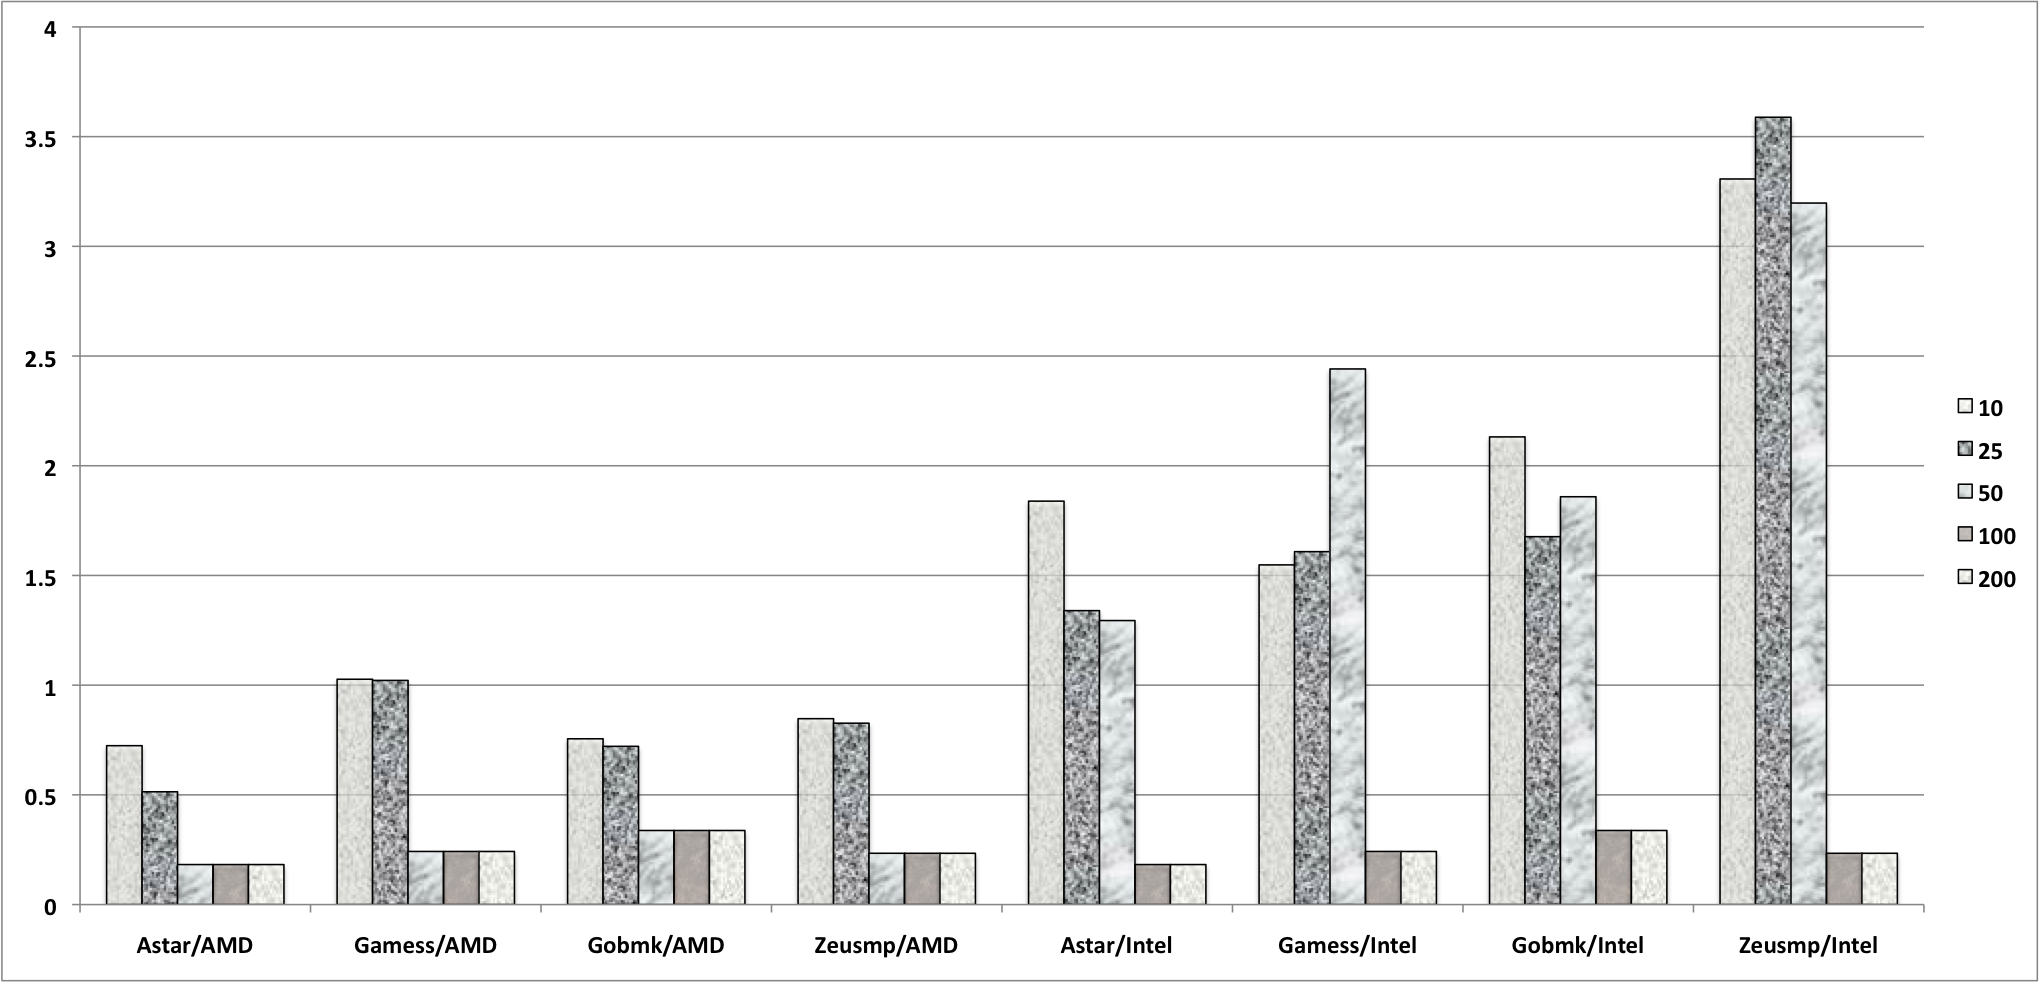
\includegraphics[width=1.0\linewidth,height=2.5in]{rmsep}
  \caption{Root Mean Square Error (RMSE) for different values of $p$.}
  \label{fig:rmsep}
\end{figure}
While the number of measures per observation ($r$) is fixed for a given
server in our evaluation (equal to 14 for the Sun Fire server and to 19
for Dell PowerEdge server), the CAP prediction time and accuracy depend
on $p$ (the number of past observations) and $n$ (the number of future
observations), as stated in Section~\ref{sec:cappcreate}.  In our
evaluation, the CAP prediction error rates of various benchmark codes
for a range of $p$ under a given $n$ were gathered, as demonstrated in
\figurename~\ref{fig:rmsep}, where $n$ equals 5.  It can be seen from
the figure that the error rates are fairly small (and stay almost
unchanged) when $p$ is within 100 to 200, but they rise considerably
when $p$ drops to 50 or below.  In subsequent figures, the prediction
results of CAP include only those for $n$ = 5 and $p$ = 100.  Each
benchmark was executed to collect the first $p$=100 points on the
attractor, at which point the next $n$=5 points were used to
compute the estimated power for the $t, t+1,\ldots,t+5$ energy estimates
in each time cycle.

\begin{figure*}[tp]
  \centering
  \subfloat[Astar/CAP.]{%
    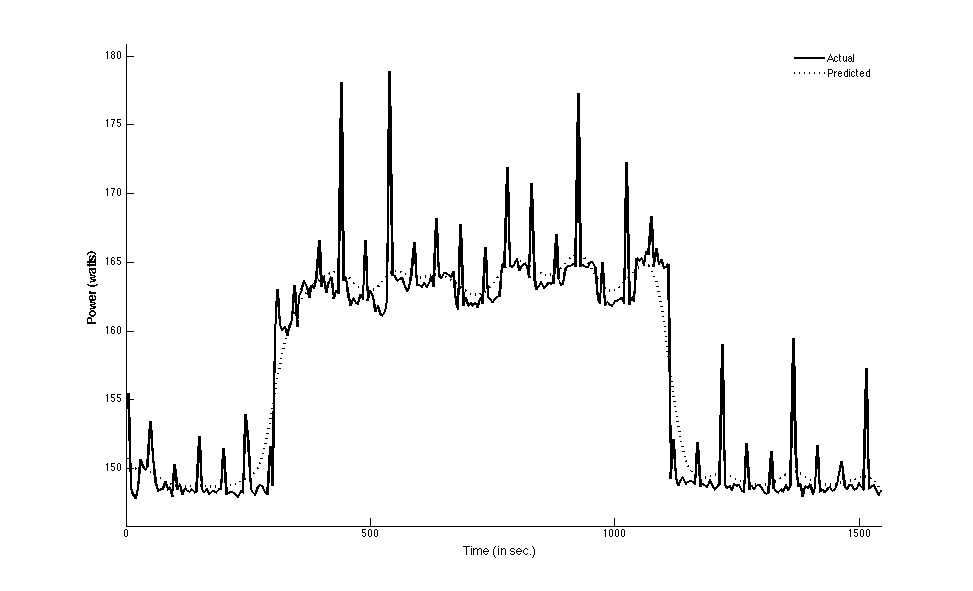
\includegraphics[width=0.5\linewidth,height=2in]{amd_ch_astar}
  }
  \subfloat[Astar/AR(1)).]{%
    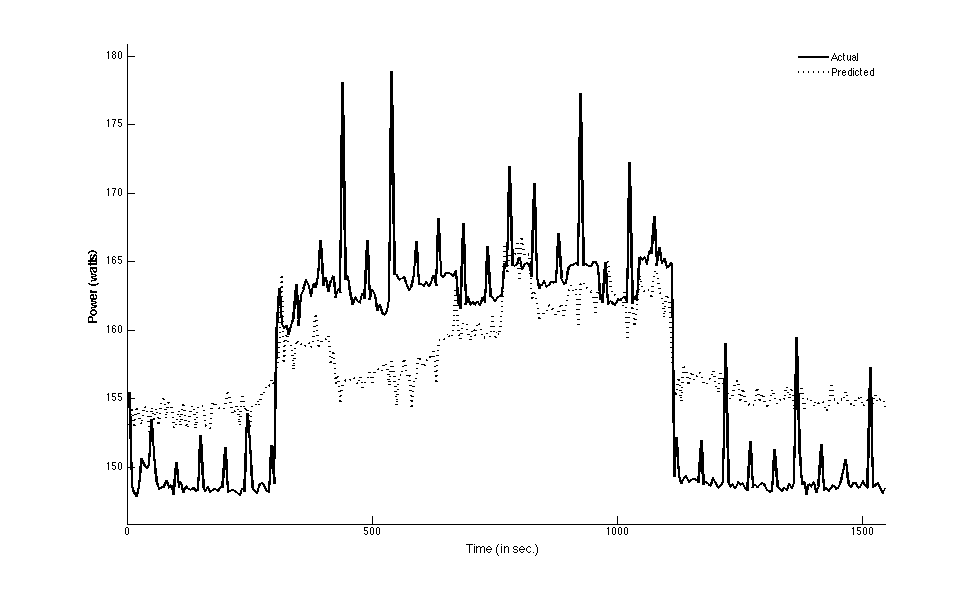
\includegraphics[width=0.5\linewidth,height=2in]{amd_ar_astar}
  }\\
  \subfloat[Zeusmp/CAP.]{%
    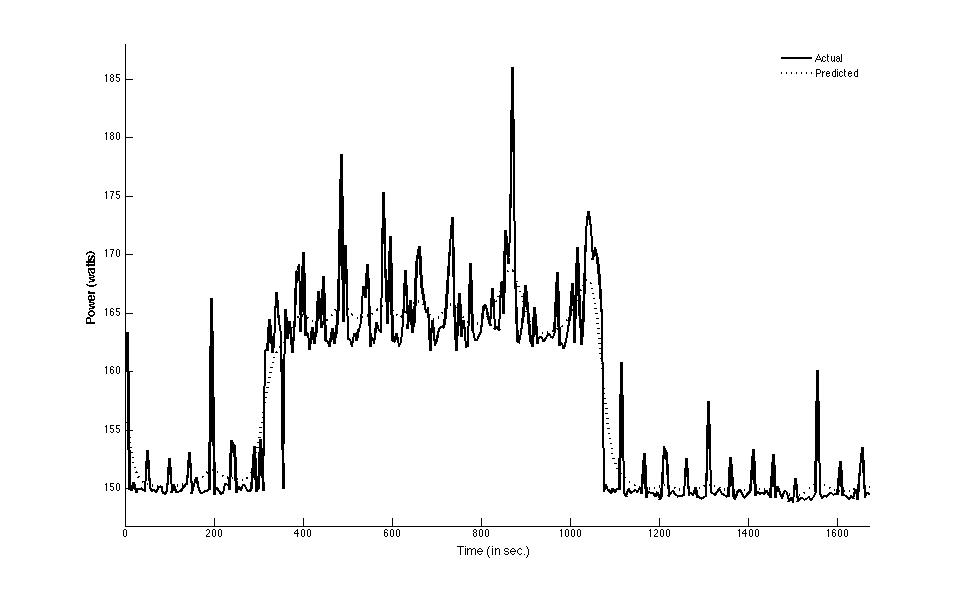
\includegraphics[width=0.5\linewidth,height=2in]{amd_ch_zeusmp}
  }
  \subfloat[Zeusmp/AR(1).]{%
    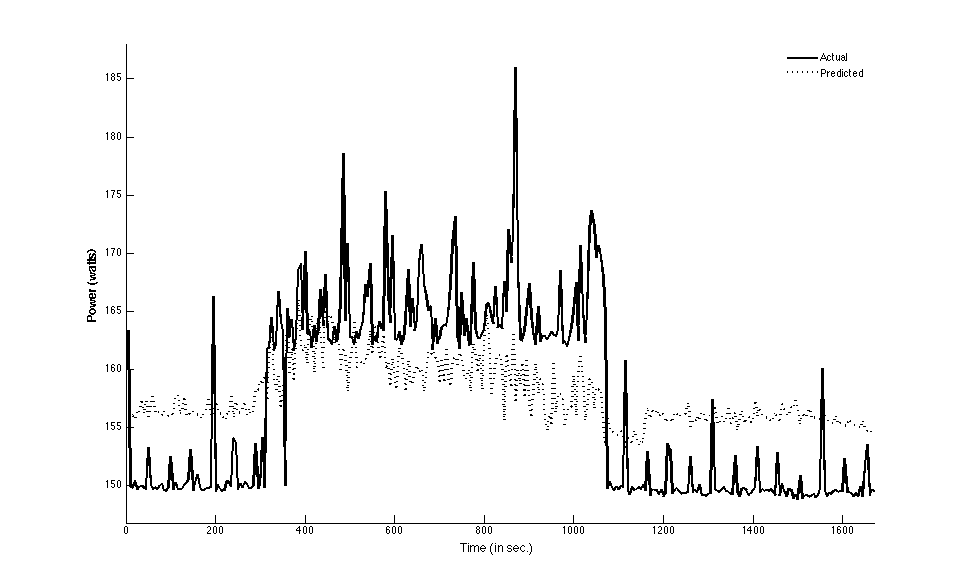
\includegraphics[width=0.5\linewidth,height=2in]{amd_ar_zeusmp}
  }
  \caption{Actual power results versus predicted results for AMD Opteron.}
  \label{fig:compareamd}
\end{figure*}
The predicted power consumption results of CAP during the execution of
Astar and Zeusmp on a HyperTransport-based server are demonstrated in
\figurenames~\ref{fig:compareamd}(a) and \ref{fig:compareamd}(c).  The
predicted values are seen to track closely to the measured readings
(obtained using the WattsUP power meter and indicated by solid curves),
with the error rate ranging between 0.9\% and 1.6\%.  For comparison,
the predicted power consumption outcomes during the execution of same
selected benchmarks under AR(1) are depicted in
\figurenames~\ref{fig:compareamd}(b) and \ref{fig:compareamd}(d), where
details of AR(1) can be found in Appendix.  As expected, AR(1) exhibits
poor outcomes over any given short execution window, with maximum errors
ranging from 7.9\% to 9.3\%, despite that the prediction error over the
whole execution period may be less.  CAP enjoys much better prediction
behavior than its linear regressive counterpart.

\begin{figure*}[tp]
  \centering
  \subfloat[Astar/CAP.]{%
    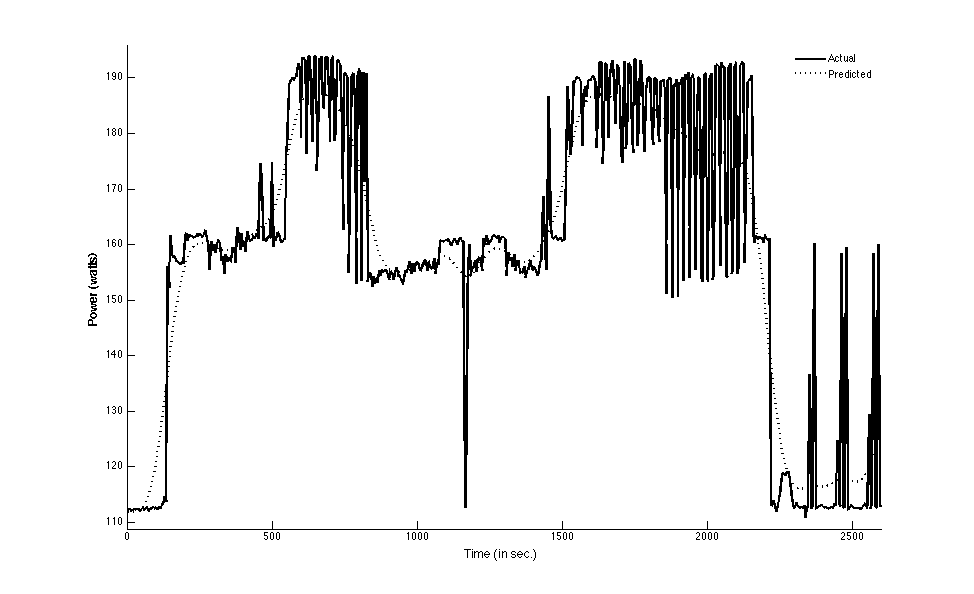
\includegraphics[width=0.5\linewidth,height=2in]{intel_ch_astar}
  }
  \subfloat[Astar/AR(1)).]{%
    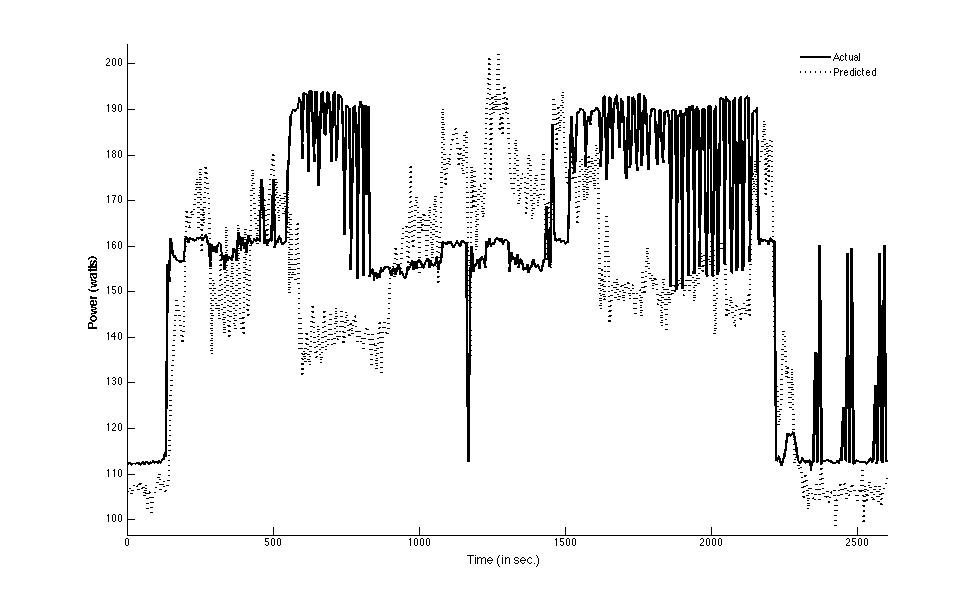
\includegraphics[width=0.5\linewidth,height=2in]{intel_ar_astar}
  }\\
  \subfloat[Zeusmp/CAP.]{%
    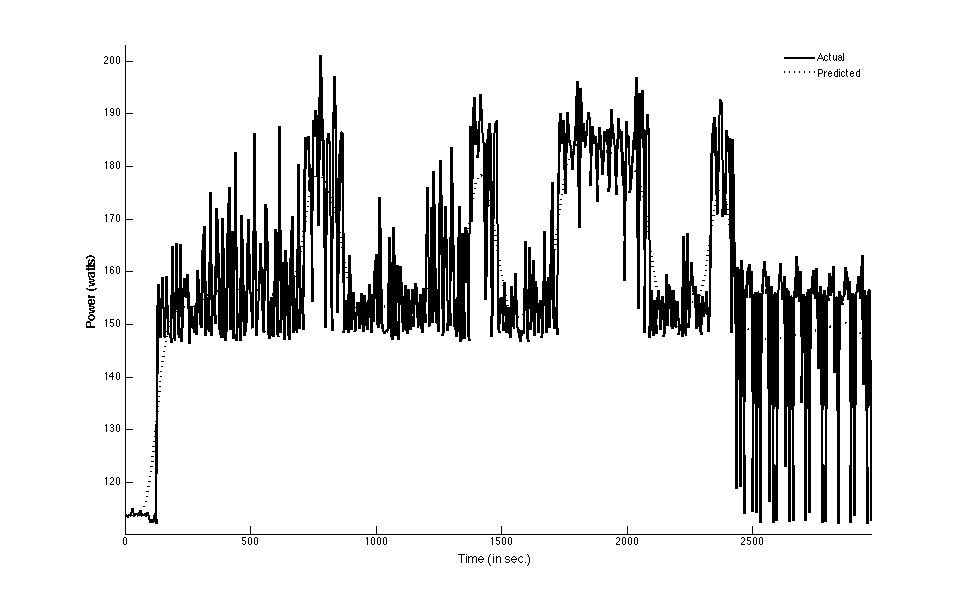
\includegraphics[width=0.5\linewidth,height=2in]{intel_ch_zeusmp}
  }
  \subfloat[Zeusmp/AR(1).]{%
    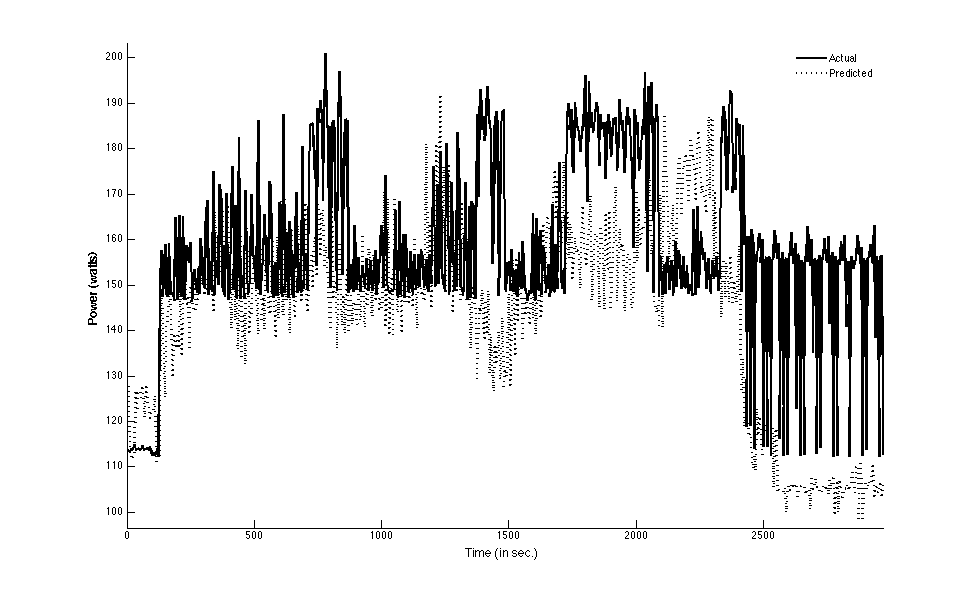
\includegraphics[width=0.5\linewidth,height=2in]{intel_ar_zeusmp}
  }
  \caption{Actual power results versus predicted results for an Intel
    Nehalem server.}
  \label{fig:compareintel}
\end{figure*}
The predicted power consumption results under CAP over the benchmark
execution period for the QPL-based server (Dell PowerEdge) are
demonstrated in \figurenames~\ref{fig:compareintel}(a) and
\ref{fig:compareintel}(c), where the actual power consumption amounts
obtained by the WattsUP meter are shown by solid curves.  Again, CAP is
seen to exhibit impressive performance, tracking the actual amounts
closely, with the error rate ranging between 1.0\% and 3.3\%.  The root
mean square errors for CAP remain within small values.  In contrast,
AR(1) suffers from poor prediction behavior, as can be discovered in
\figurenames~\ref{fig:compareintel}(b) and \ref{fig:compareintel}(d),
where outcomes of same benchmarks executed on the Dell PowerEdge server
are depicted.  It yields the maximum error up to 20.8\% (or 20.6\%) for
the Astar (or Zeusmp) benchmark.  
{\addtolength{\tabcolsep}{-3pt}
\begin{table}%[tbhp]
  \tbl{Model errors for CAP (under $n=5$, $p=100$, $r=19$), AR, MARS, and
    EWMA predictors on Intel Nehalem server\label{tab:modelerroroptIntel}}}&\multicolumn{1}{c}{\textbf{Err \%}}&\multicolumn{1}{c|}{}&\multicolumn{1}{c}{\textbf{Err \%}}&\multicolumn{1}{c}{\textbf{Err \%}}&\multicolumn{1}{c }{\textbf{}}\\
      \hline
      Astar &1.1\%&20.8\%&1.83&5.9\%&28.5\%&4.94\\
      Gamess &1.0\%&14.8\%&1.54&5.6\%&44.3\%&5.54\\
      Gobmk &1.0\%&21.5\%&2.13&5.3\%&27.8\%&4.83\\
      Zeusmp&3.3\%&20.6\%&3.31&7.7\%&31.8\%&7.24\\
      \hline
      \multicolumn{1}{c|}{}&\multicolumn{3}{c|}{\textbf{MARS}}&\multicolumn{3}{c}{\textbf{EWMA}}\\
      \hline
  &\multicolumn{1}{c}{\textbf{Avg}}&\multicolumn{1}{c}{\textbf{Max}}&\multicolumn{1}{c|}{\textbf{RMSE}}&\multicolumn{1}{c}{\textbf{Avg}}&\multicolumn{1}{c}{\textbf{Max}}&\multicolumn{1}{c}{\textbf{RMSE}}\\
\multicolumn{1}{c|}{\textbf{Benchmark}}&\multicolumn{1}{c}{\textbf{Err \%}}&\multicolumn{1}{c}{\textbf{Err \%}}&\multicolumn{1}{c|}{}&\multicolumn{1}{c}{\textbf{Err \%}}&\multicolumn{1}{c}{\textbf{Err \%}}&\multicolumn{1}{c }{\textbf{}}\\
      \hline
      Astar &5.4\%&28.0\%&4.97&3.7\%&32.4\%&2.98\\
      Gamess &4.7\%&33.0\%&4.58&1.8\%&27.3\%&2.19\\
      Gobmk &4.1\%&27.9\%&4.73&3.9\%&28.4\%&2.73\\
      Zeusmp&11.6\%&32.2\%&8.91&5.0\%&31.3\%&2.81\\
      \hline
    \end{tabular}}
  \end{table}
}

\subsection{Further discussion}
\label{sec:caseanalysis}
Tables~\ref{tab:modelerroropt} (or \ref{tab:modelerroroptIntel})
compares the errors of evaluation benchmarks for the server with the
HyperTransport (or QPL) structure, under four different prediction
mechanisms: CAP, AR, MARS, and EWMA.  Details of AR, MARS, and EWMA
predictors can be found in Appendix.  Large errors exhibited by AR,
MARS, and EWMA overwhelm the advantages gained from their simplicity.
The table results indicate the limitations entailed by using a linear
technique, such as AR time series, to predict dynamic system behavior;
similar issues exist for piecewise and moving average techniques, such as
MARS and EWMA.  Earlier attempts were made to address this issue by
incorporating corrective mechanisms in combination with these
predictors.  An example attempt employed machine learning to monitor 
mis-prediction, with recalibration invoked when required
\cite{Coskun2008}.  CAP eliminates the need for any corrective mechanism
by directly addressing the system dynamics, thereby avoiding wide drifts in
prediction experienced by other prediction techniques.

The model developed in this paper is valid for any
dual-core/dual-processor system using NUMA memory access connected in a
point-to-point manner using the HyperTransport or the QPL structures.
However, it can be scaled to quad-core dual processors based on those
two structures.  One would expect to see a slight difference or
variation in power prediction due to a greater or less affect of die
temperatures on the other performance measures.  Under a dual-core
quad-processor server, for example, additional regression variables
would be incorporated in $E_{proc}$, giving rise to more performance
measures (i.e., a larger $r$).  Similarly, more PeCs related to cache
misses would then be involved in $E_{mem}$.  The solution approach of
CAP remains exactly identical, except for a larger $r$ in its prediction
computation.

The experimental validation of CAP reveals opportunities for further
investigation.  CAP has been validated for NUMA-based servers, built on
AMD Operton processors and Intel Xeon processors with Nehalem
architecture; it requires validation on other architectures, like NVIDA
GPU processors and IBM Cell BE processors.  Further studies on the power
and thermal envelope of multi-chip server systems, which involve network
traffic and off-chip synchronization traffic, is required to understand
their contributions to the system thermal envelope.
\section{Conclusion}
\label{sec:conclusions}
A fast and accurate model for energy consumption and thermal envelope in
a server is critical to understanding and solving the power management
challenges unique in dense servers.  In this paper, we have introduced a
comprehensive model of energy consumption by servers as a continuous
system of differential equations.  The model measures energy input to
the system as a function of the work done for completing tasks being
gauged and the residual thermal energy given off by the system as a
result.  Traffic on the system bus, misses in the L2 cache, CPU
temperatures, and ambient temperatures are combined together to create a
model, which can be employed to manage the processor thermal envelope.

The model serves as a predictive tool by approximating observed
performance metrics in a discrete time series for estimating future
metrics, and thus corresponding energy consumption amounts.  It was
found through experimental validation that commonly used techniques of
regressive time series forecasting, while attractive because of their
simplicity, inadequately capture the non-linear and chaotic dynamics of
metric readings for typical server systems.  Therefore, a chaotic time
series approximation for run-time power consumption is adopted to arrive
at Chaotic Attractor Prediction (CAP), which exhibits polynomial time
complexity.  Our proposed model is the first step towards building
solutions for power and thermal management in data centers usually
housing many servers.
\appendix
\section*{APPENDIX}
\setcounter{section}{1} 
This appendix describes three regression-based prediction models: a linear
AR(1) model \cite{Box1994}, a MARS model \cite{Friedman1991}, and an
EWMA model. 
Each model is an  approximations to the dynamic system in
\equationname~(\ref{eq:linmodel}), following regressive combinations of
five energy contributors to a server, as given in 
\equationname~(\ref{eq:tseries})~\cite{Lewis2008}.

The same data sets used to generate the chaotic model were used to
create the AR(1) model. Two methods were considered for consolidation:
arithmetic mean (average) and geometric mean.  Trial models were
constructed using each method and a statistical analysis of variance was
performed to determine which model generated the best fit to the
collected data with a time interval $t=5$ seconds.  Note that the statistical coefficients need to be computed
only once using some benchmarks, for a given server architecture.
The coefficients obtained can then be provided through either
the system firmware or the operating system kernel for use in the server
executing any application.

Under linear auto-regression, energy consumed by the processor for the
AMD server, $E_{proc}^{AMD}$ as defined by
\equationname~(\ref{eq:procpwr2}), is a \textit{linear combination} of
$MP_{proc}^{AMD}$ measures (stated in Section~\ref{sec:variables}) as \cite{Lewis2008}:
\begin{equation*}
  \label{eq:apxproc}
  E_{proc}^{AMD} \approx 0.49*T_{C_{0}}+0.50*T_{C_{1}}+0.01*HT_{1}. 
\end{equation*}

For the Intel server, its energy consumption by the processor,
$E_{proc}^{Intel}$, is a function of $MP_{proc}^{Intel}$ (detailed in
Section~\ref{sec:variables}), leading to its estimated energy as follows:
\begin{equation*}
  \label{eq:apxpr}
  E_{proc}^{Intel} \approx 2.29*T_{C_{0}}+0.03*T_{C_{1}}+0.52*QPL_{C}.
\end{equation*}
 
In a similar fashion, energy consumed by the memory subsystem in the AMD server,
$E_{mem}^{AMD}$, is a function of $MP_{mem}^{AMD}$, yielding
\begin{equation*}
  \label{eq:apxmem}
  E_{mem}^{AMD} \approx 0.01*HT_{2}+0.003*CM_{0}+0.003*CM_{1}+0.014*CM_{2}+0.01*CM_{3}.
\end{equation*}

Energy consumption for the memory subsystem in the Intel server,
$E_{mem}^{Intel}$, is a function of $MP_{mem}^{Intel}$, giving rise to
\begin{equation*}
  E_{mem}^{Intel} \approx 0.52*QPL_{IO}+0.35*CM_{0}+0.31*CM_{1}. 
\end{equation*}

Energy consumed as a result of disk activities in the AMD server (or the
Intel server) is a function of $MP_{hdd}^{AMD}$ (or $MP_{hdd}^{Intel}$),
arriving at 
\begin{equation*}
E_{hdd}^{AMD} \approx 0.014*D_{r}+0.007*D_{w}
\end{equation*}
and
\begin{equation*}
E_{hdd}^{Intel} \approx 0.01*D_{r}+0.01*D_{w}.
\end{equation*}

Energy consumed by the board in the AMD server is a function of $MP_{board}^{AMD}$,
whose components are added in a linearly weighted fashion to derive
$E_{board}^{AMD}$ (or $E_{board}^{Intel}$), as follows:
\begin{equation*}
E_{board}^{AMD} \approx 0.101+0.81*T_{A_{0}}+0.62*T_{A_{1}}
\end{equation*}
and
\begin{equation*}
E_{board}^{Intel} \approx 2.53+0.03*T_{A_{0}}+0.01*T_{A_{1}}+0.01*T_{A_{2}}.
\end{equation*}

Finally, energy consumed by electromechanical elements in the AMD server, $E_{em}^{AMD}$,
is a linear function of $MP_{em}^{AMD}$, leading to
\begin{equation*}
E_{em}^{AMD} \approx 0.001*F_{C}+0.001*F_{M}.
\end{equation*}
Similarly, energy consumption attributed to electromechanical elements in the Intel server, $E_{em}^{Intel}$, equals
\begin{align*}
E_{em}^{Intel}\approx4.85*F_{C}&+6.61*F_{M2a}+3.92*F_{M2b}+0.28*F_{M3a}+0.52*F_{M3b}\\
            &+0.01*F_{M4a}+0.01*F_{M4b}+0.78*F_{M5a}+0.61*F_{M5b}.
\end{align*}

Total energy consumption for the AMD server (or the Intel server)
under AR(1) equals the summation of above five consumption contributors
\cite{Lewis2008}.

The models for AMD and Intel severs reveal the issues of adopting linear
regression to obtain individual component contribution.  Consider the
Intel processor as an example.  The coefficients for temperature sensors
are significantly larger than those for the workload-related PeCs, with
those coefficients apparently overbalancing the remaining model
components.  This fact is quite non-intuitive, as one would like to
derive certain physical interpretation on each constant to understand
the behavior of its associated model component.  In addition, other
processor models have negative coefficients for similar model
components, making linear regression deemed unsuitable for such modeling
~\cite{Bertran2010,McCullough2011}.

The MARS predictor used in our evaluation was created using the
consolidated data set employed to establish the CAP and the AR(1)
predictors.  It was generated by means of the ARESlab toolkit
\cite{Jekabsons2010}, and the resulting set of splines served as a
predictive tool, as described in Section~\ref{sec:evaluation}.  Note
that ARESlab is a MATLAB toolkit for building piecewise-linear and
piecewise-cubic MARS regression models.  The toolkit was adopted to
build a piece-wise cubic model using the same consolidated training set
employed for creating the AR and the CAP models.  The toolkit output is
a structure which defines the basis functions and associated
coefficients of \equationname~(\ref{eq:mars}) given in
Section~\ref{sec:priorwork} to approximate system dynamics.

The EWMA predictor used in our evaluation was also created using the
consolidated data set employed to established CAP, AR(1), and MARS
predictors.  The predictor was generated using an Exponentially Weighted
Moving Average using the recurrence relation of
\begin{align}
  \label{eq:1}
  S_{1}&=Y_{1}\nonumber\\
  S_{t}&=\alpha Y_{t-1}+(1-\alpha))S_{t-1}, t>1\nonumber
\end{align}
where $Y_{t}$ is an observation of the power consumed at time $t$,
$S_{t}$ is the value of the weighted average at time $t$, and $\alpha$
is a coefficient representing the weighting decrease degree, for
$0\leq \alpha \leq1$.

\label{sec:references}
\bibliographystyle{acmsmall}
\bibliography{powermodel.bib}

\received{December 2010}{August 2011, December 2011}{May 2012}

\end{document}
% The following comment block is used by the different flavors of EMACS and
% to set file-local configuration variables.  They are required 
% to guarantee correct behavior of EMACS, AUCTEX, and LaTeX.
%
% Please do not remove.
%%% Local Variables: 
%%% mode: latex flyspell
%%% TeX-master: "powermodel.tex"
%%% TeX-PDF-mode: t
%%% End: 

